\chapter{Recherche de résonances de spin 0 -- comparaisons données / simulation} \label{an:higgs_data_mc}

Cette annexe présente les comparaisons données / simulation non incluses dans le \cref{chap:higgs}, pour l'impulsion transverse du lepton sélectionné (\cref{fig:higgs_data_mc_lepton}), pour l'impulsion transverse du premier jet sélectionné (\cref{fig:higgs_data_mc_1jet}), pour l'énergie transverse manquante (\cref{fig:higgs_data_mc_met}) ainsi que pour le nombre de jets étiquetés \Pbottom (\cref{fig:higgs_data_mc_nb}).

\begin{figure}[p!] \centering
    \captionsetup{format=plain,indention=0.2cm,font=small,labelfont={sf,bf},justification=centering}
    \subcaptionbox{Canal semi-muonique,\\au moins 2 jets étiquetés \Pbottom}[0.49\textwidth]{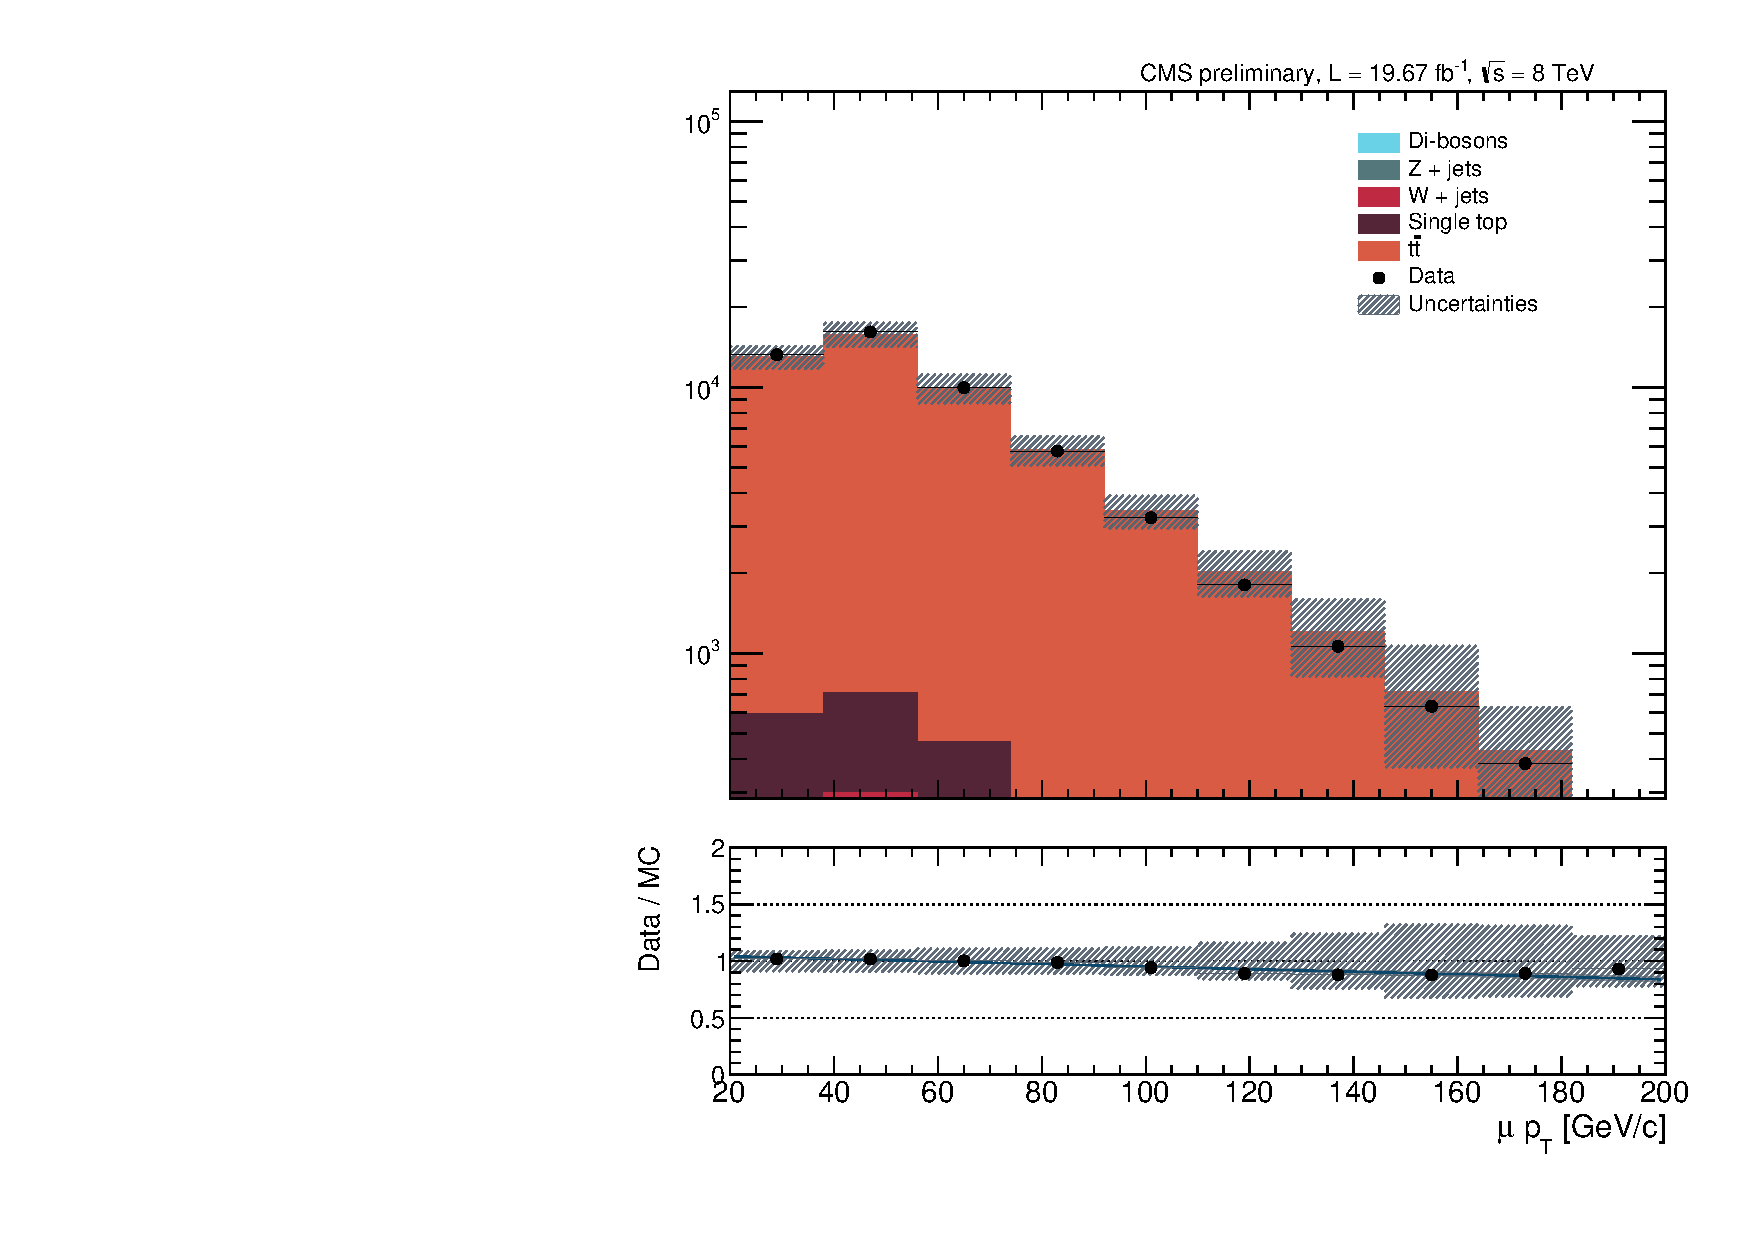
\includegraphics[width=0.49\textwidth,angle=-90,origin=c]{annexes/figs/higgs/data_mc/2-btag/semimu/leptonPt_reco_fullsel.pdf}} \hfill
    \subcaptionbox{Canal semi-électronique,\\au moins 2 jets étiquetés \Pbottom}[0.49\textwidth]{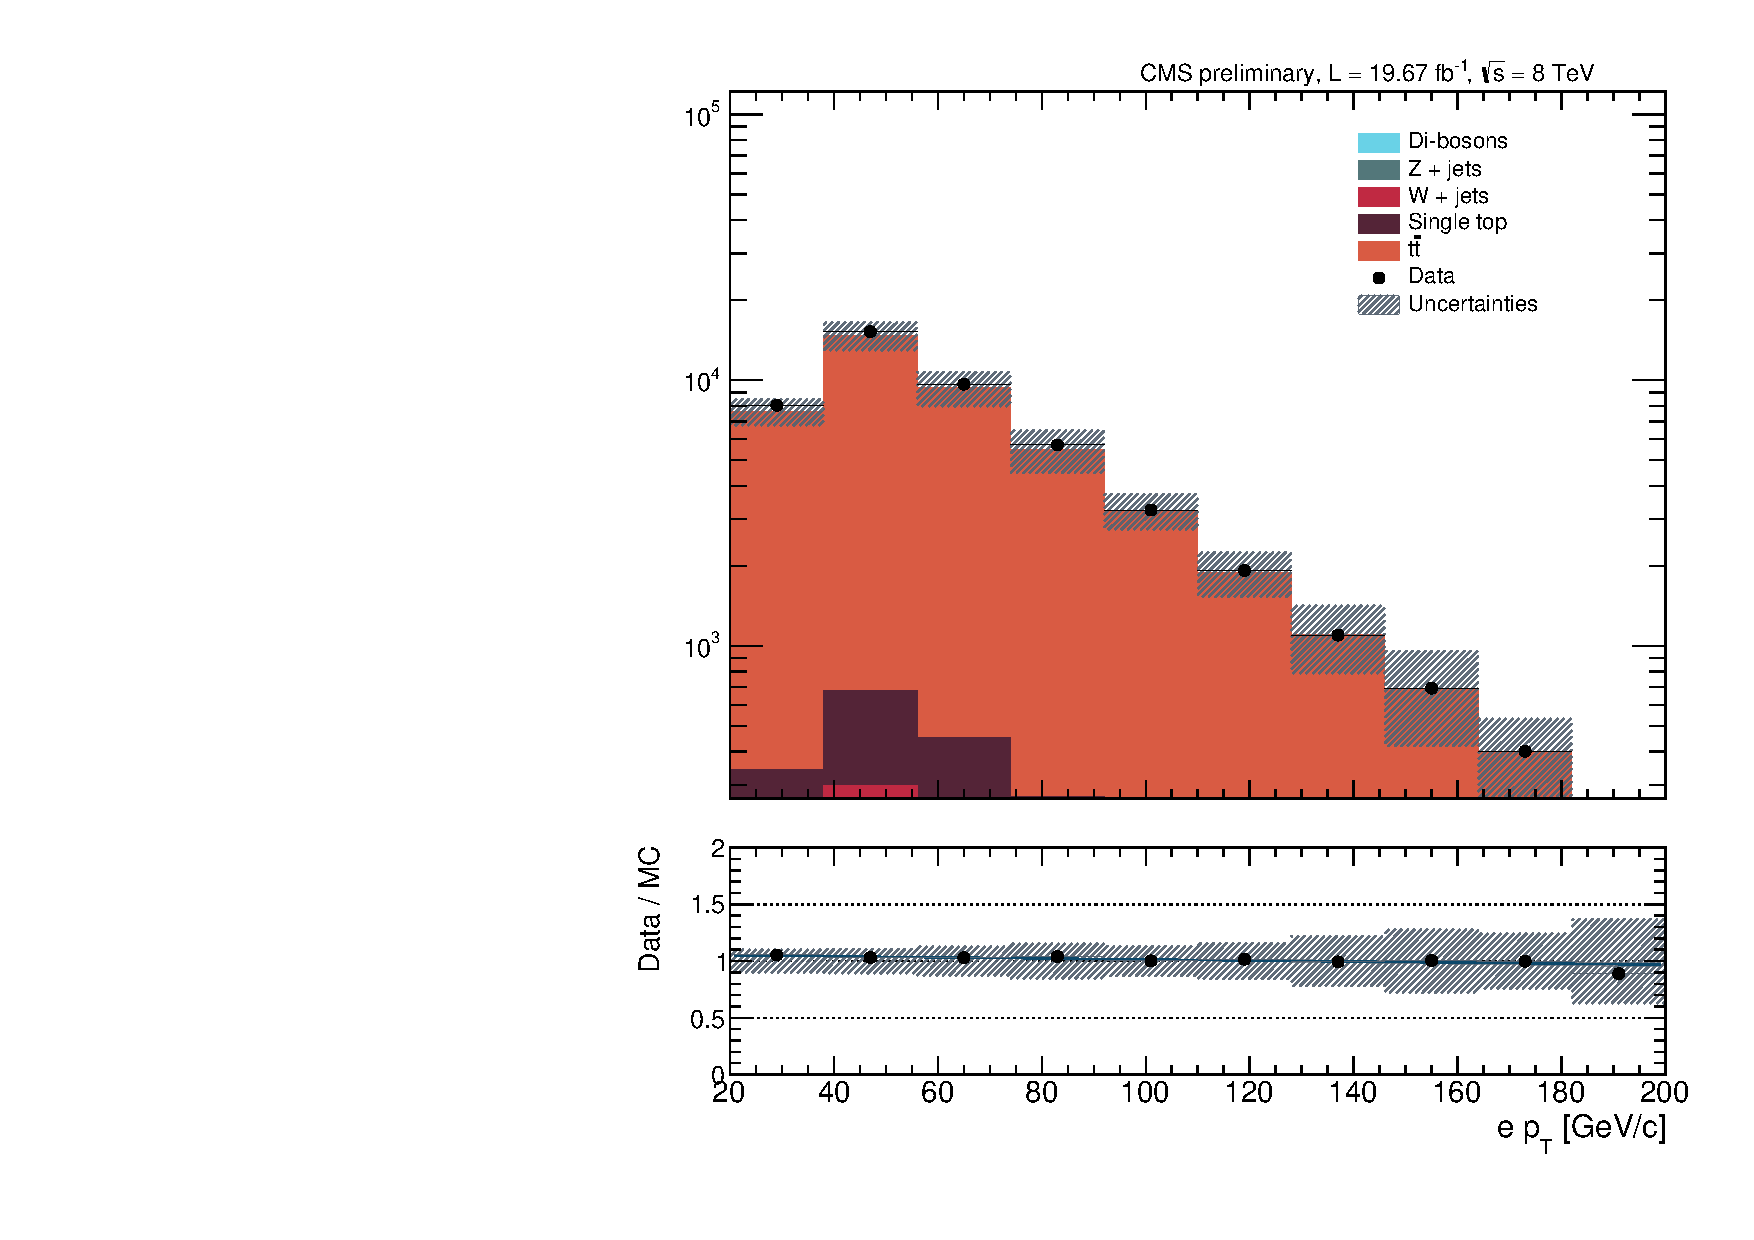
\includegraphics[width=0.49\textwidth,angle=-90,origin=c]{annexes/figs/higgs/data_mc/2-btag/semie/leptonPt_reco_fullsel.pdf}} \\ \vspace{5mm}
    \subcaptionbox{Canal semi-muonique,\\exactement 1 jet étiqueté \Pbottom}[0.49\textwidth]{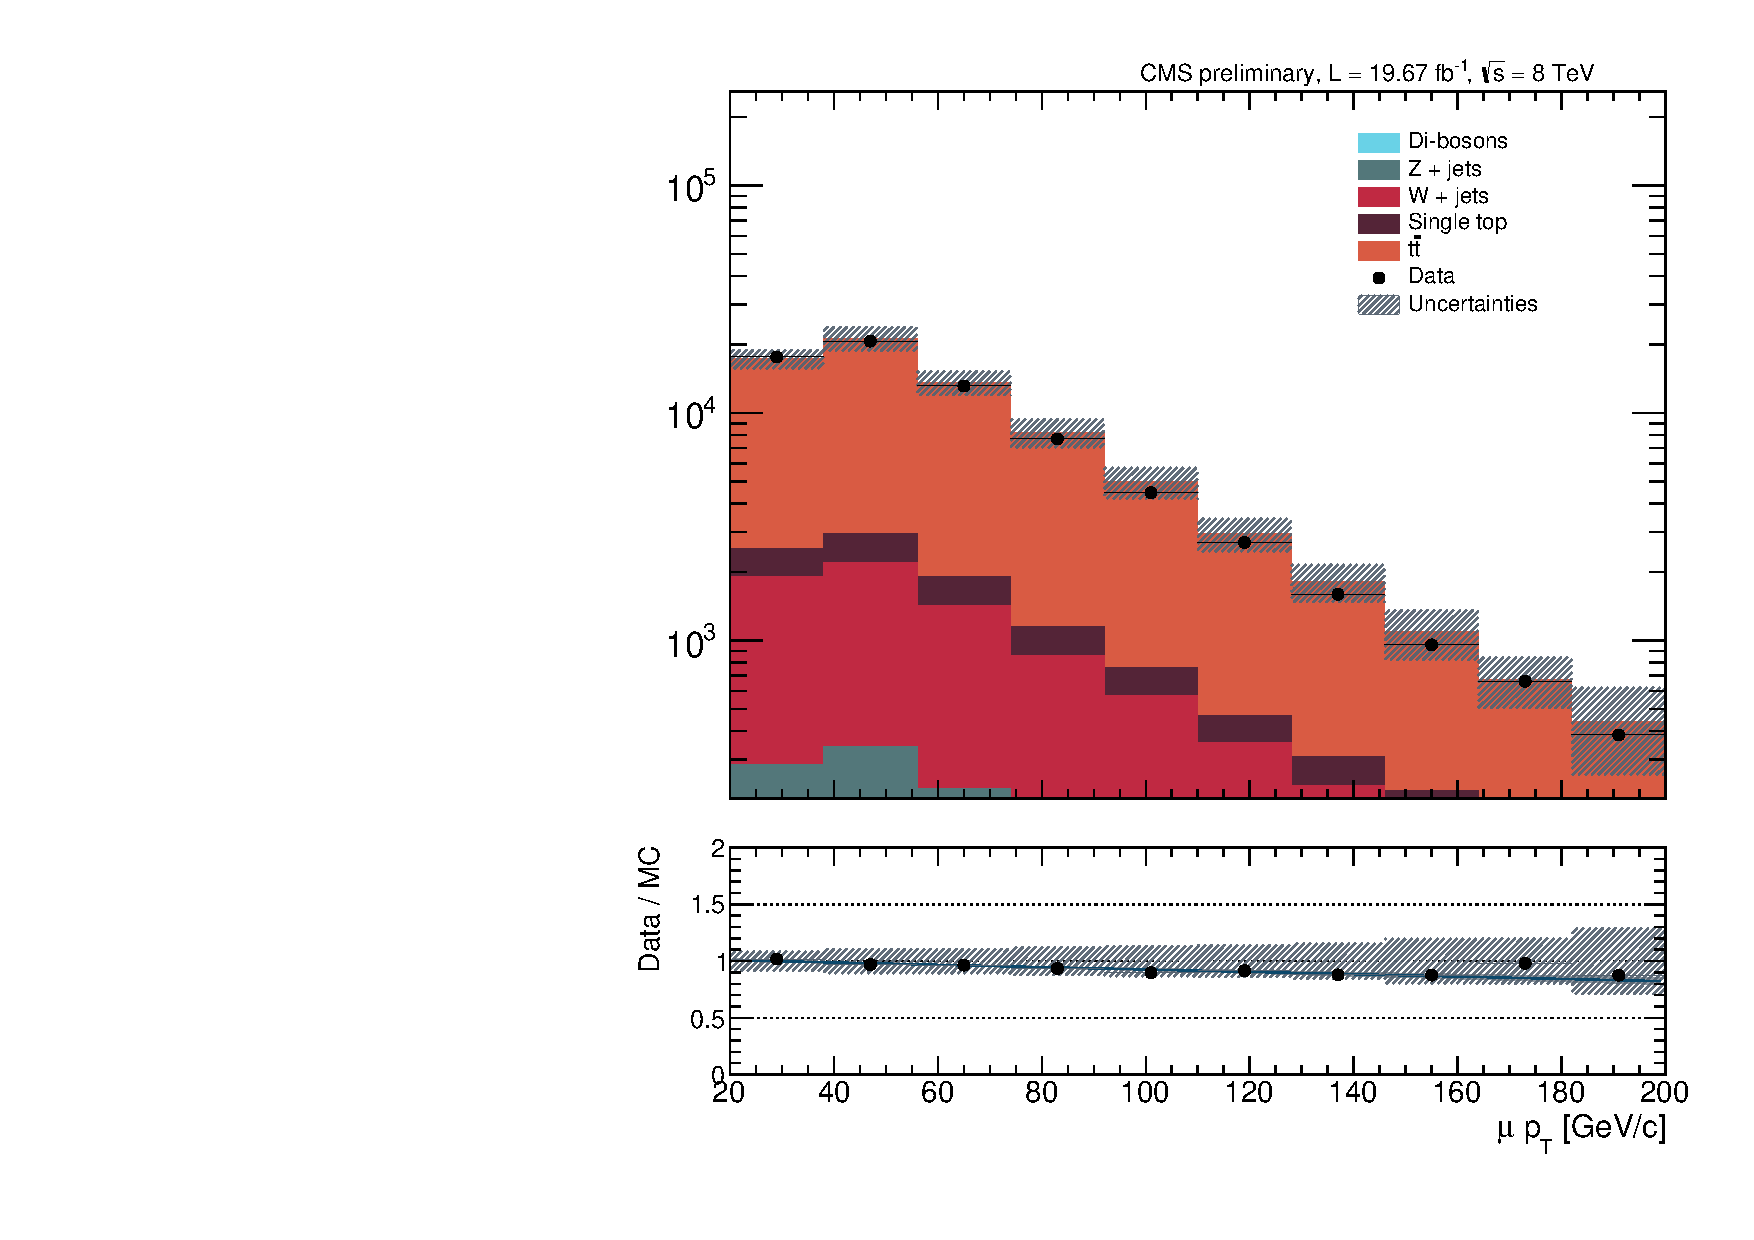
\includegraphics[width=0.49\textwidth,angle=-90,origin=c]{annexes/figs/higgs/data_mc/1-btag/semimu/leptonPt_reco_fullsel.pdf}} \hfill
    \subcaptionbox{Canal semi-électronique,\\exactement 1 jet étiqueté \Pbottom}[0.49\textwidth]{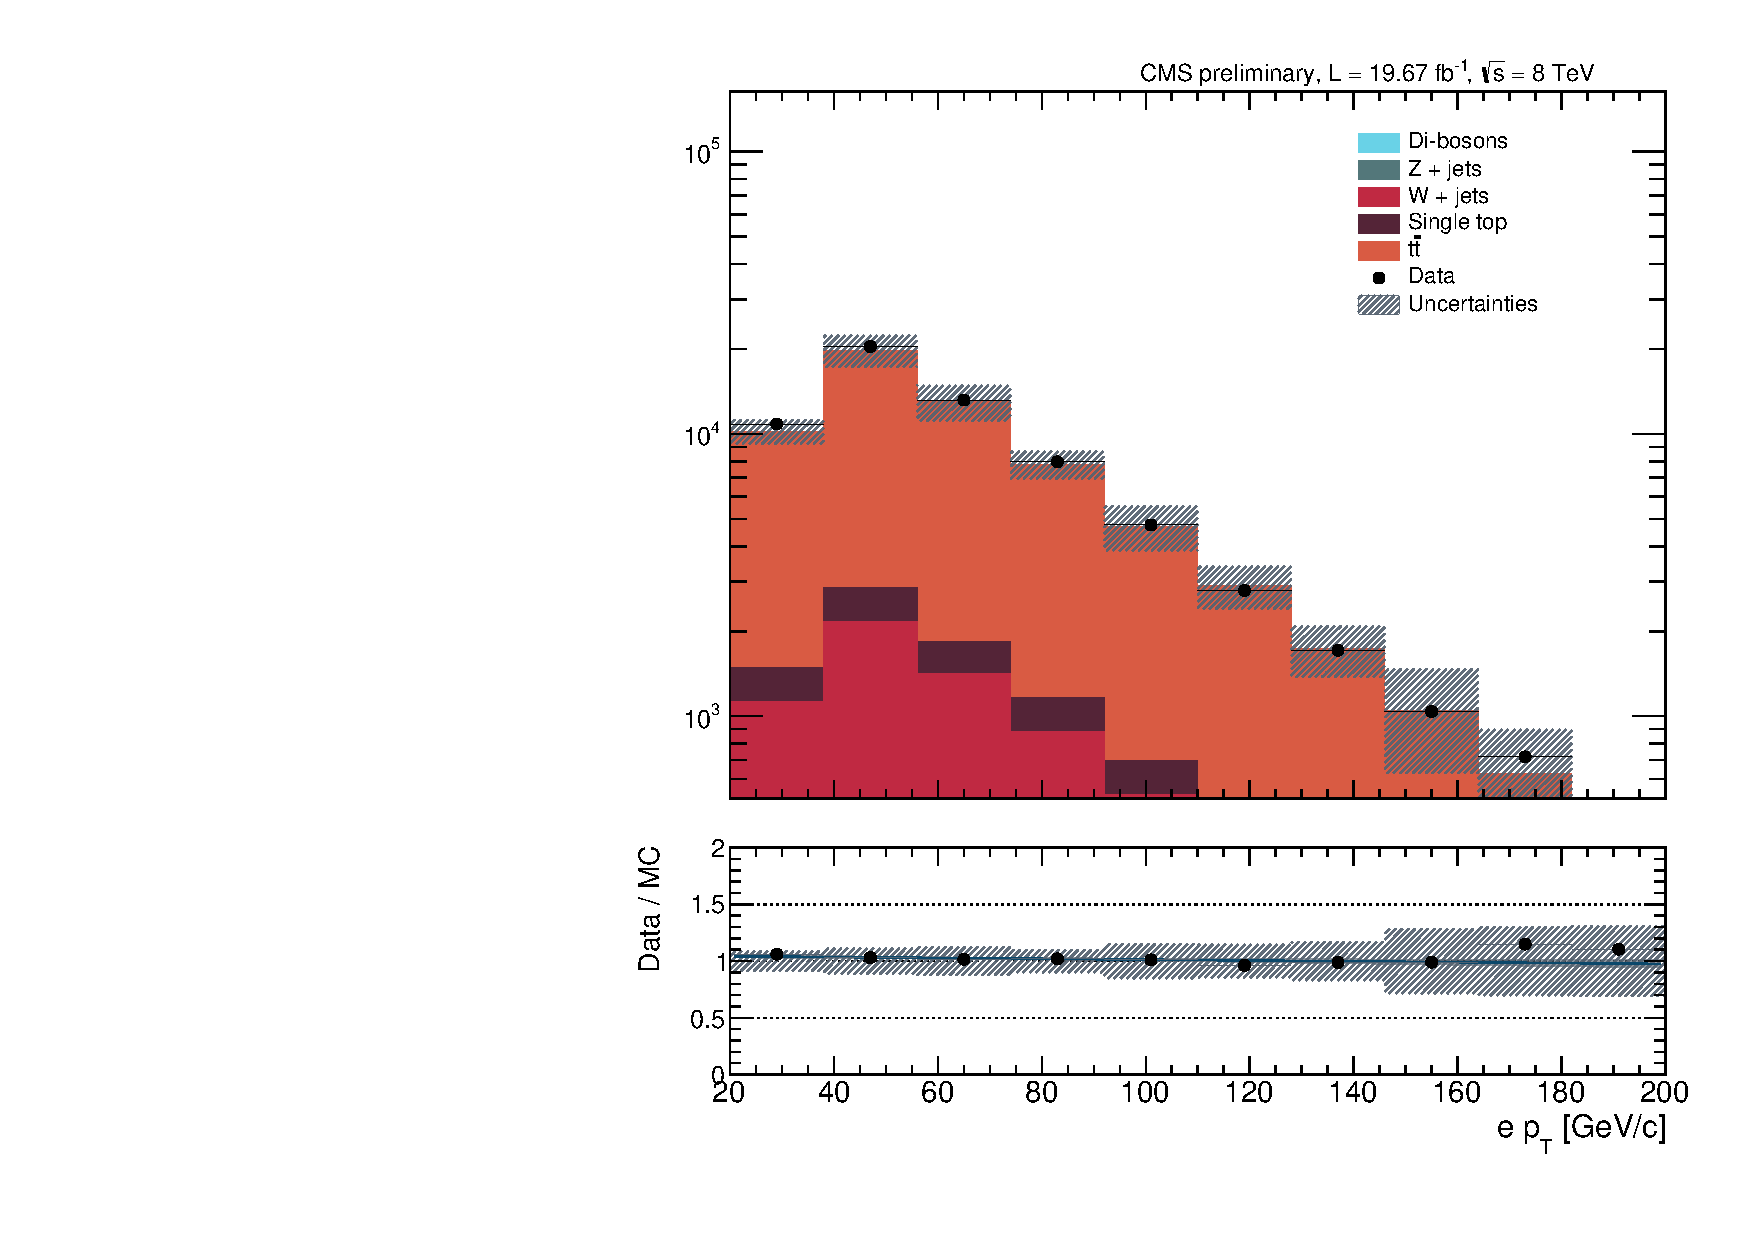
\includegraphics[width=0.49\textwidth,angle=-90,origin=c]{annexes/figs/higgs/data_mc/1-btag/semie/leptonPt_reco_fullsel.pdf}}
    \captionsetup{format=plain,indention=0.2cm,font=small,labelfont={sf,bf},justification=justified}
    \caption{Comparaison entre les données et la simulation de l'impulsion transverse du lepton sélectionné. Un ratio est présenté en bas de la distribution. La simulation est normalisée au nombre d'événements dans les données, en utilisant des facteurs de correction extraits d'un ajustement par la méthode du maximum de vraisemblance. La zone hachurée correspond aux incertitudes statistiques + systématiques.}
    \label{fig:higgs_data_mc_lepton}
\end{figure}

\begin{figure}[p!] \centering
    \captionsetup{format=plain,indention=0.2cm,font=small,labelfont={sf,bf},justification=centering}
    \subcaptionbox{Canal semi-muonique,\\au moins 2 jets étiquetés \Pbottom}[0.49\textwidth]{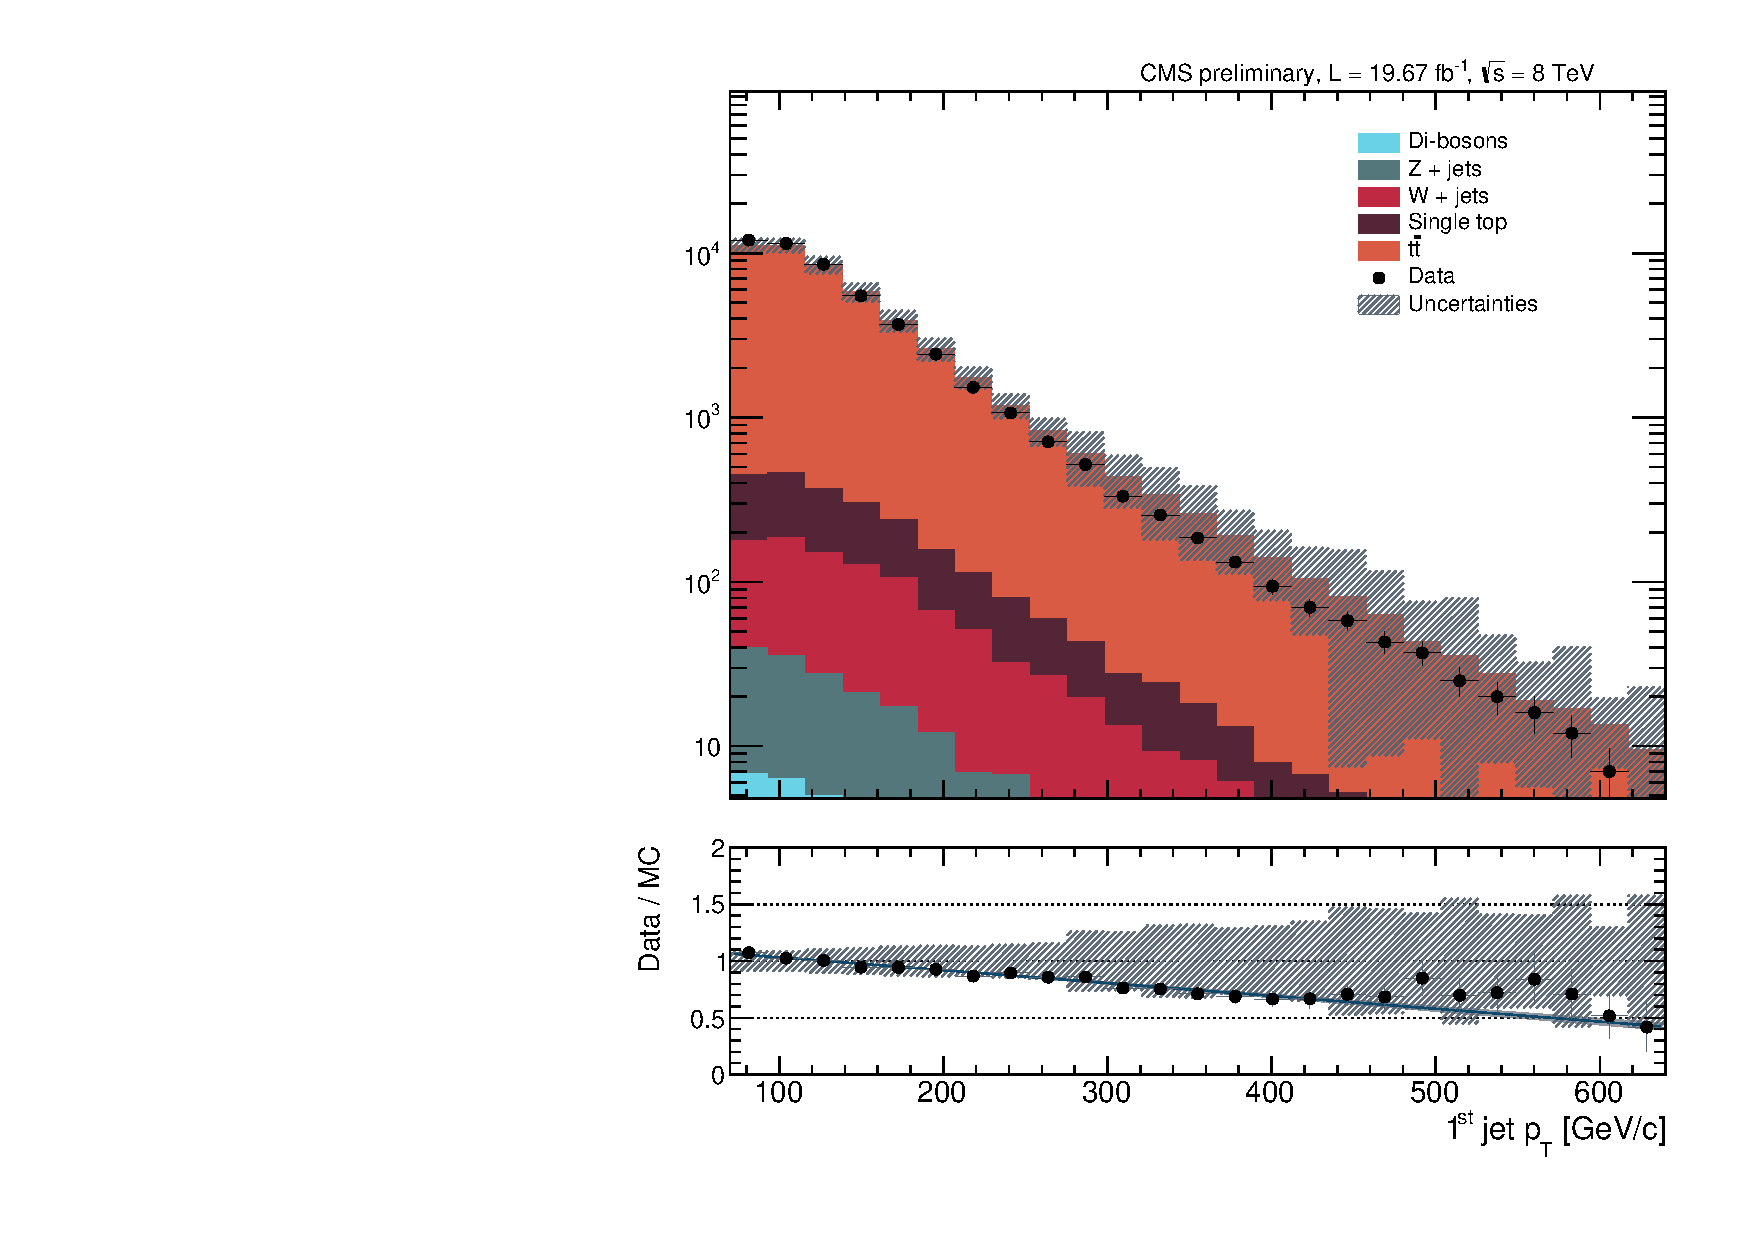
\includegraphics[width=0.49\textwidth,angle=-90,origin=c]{annexes/figs/higgs/data_mc/2-btag/semimu/firstJetPt_reco_fullsel.pdf}} \hfill
    \subcaptionbox{Canal semi-électronique,\\au moins 2 jets étiquetés \Pbottom}[0.49\textwidth]{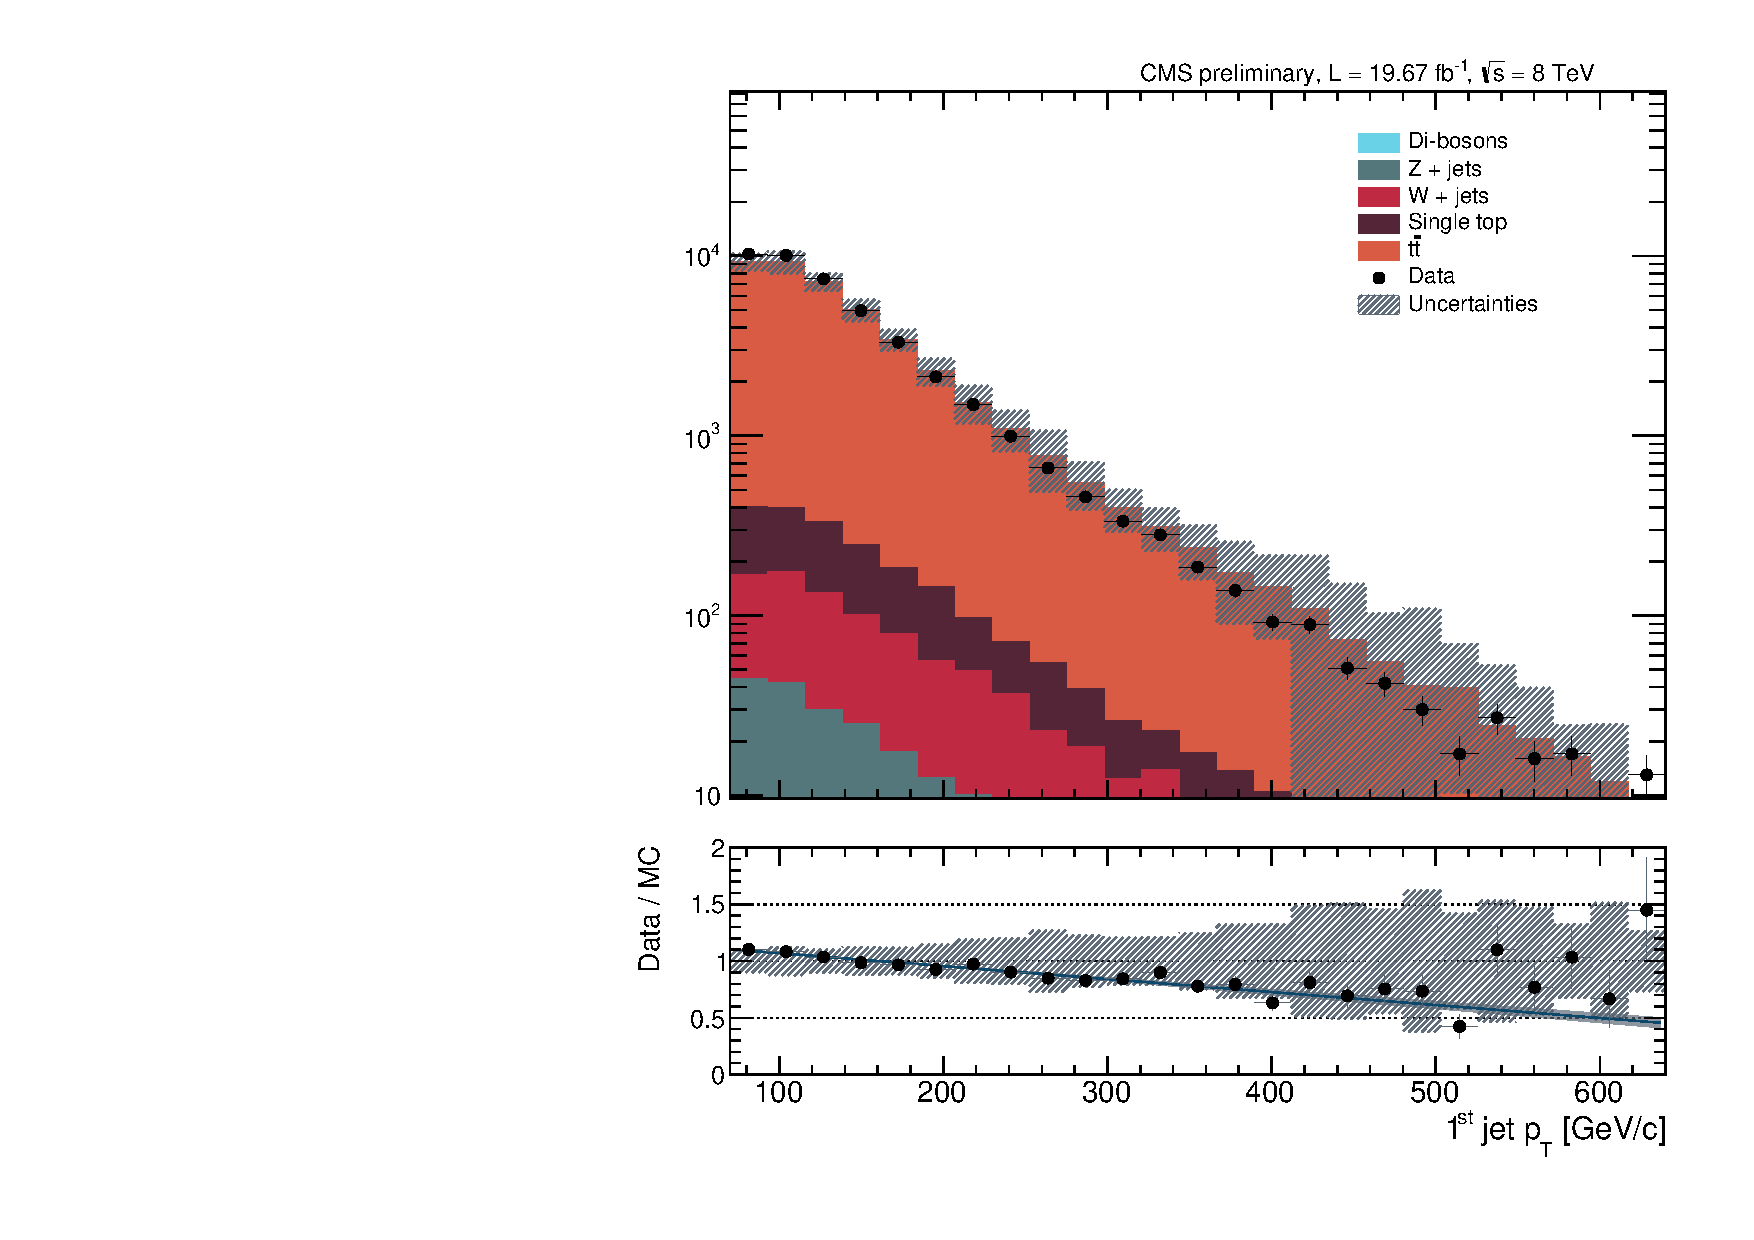
\includegraphics[width=0.49\textwidth,angle=-90,origin=c]{annexes/figs/higgs/data_mc/2-btag/semie/firstJetPt_reco_fullsel.pdf}} \\ \vspace{5mm}
    \subcaptionbox{Canal semi-muonique,\\exactement 1 jet étiqueté \Pbottom}[0.49\textwidth]{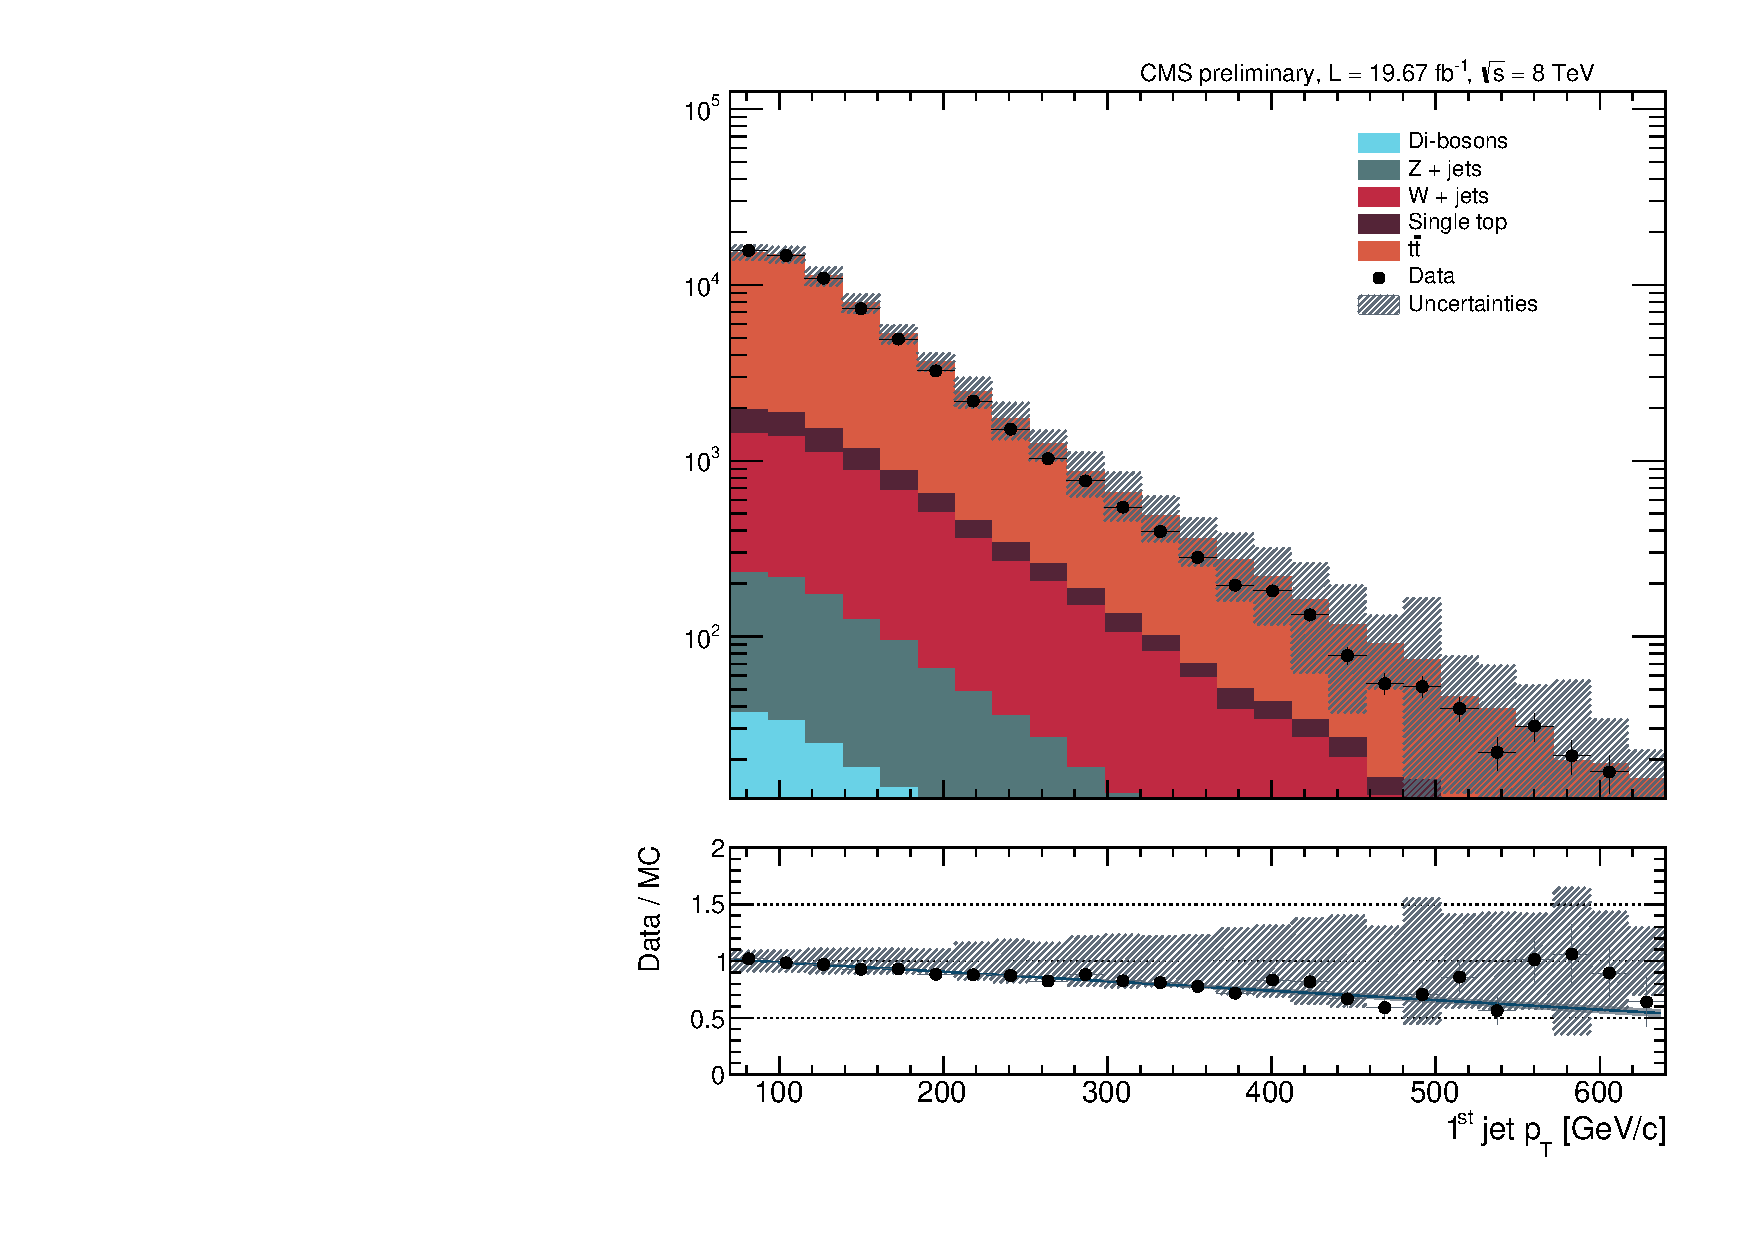
\includegraphics[width=0.49\textwidth,angle=-90,origin=c]{annexes/figs/higgs/data_mc/1-btag/semimu/firstJetPt_reco_fullsel.pdf}} \hfill
    \subcaptionbox{Canal semi-électronique,\\exactement 1 jet étiqueté \Pbottom}[0.49\textwidth]{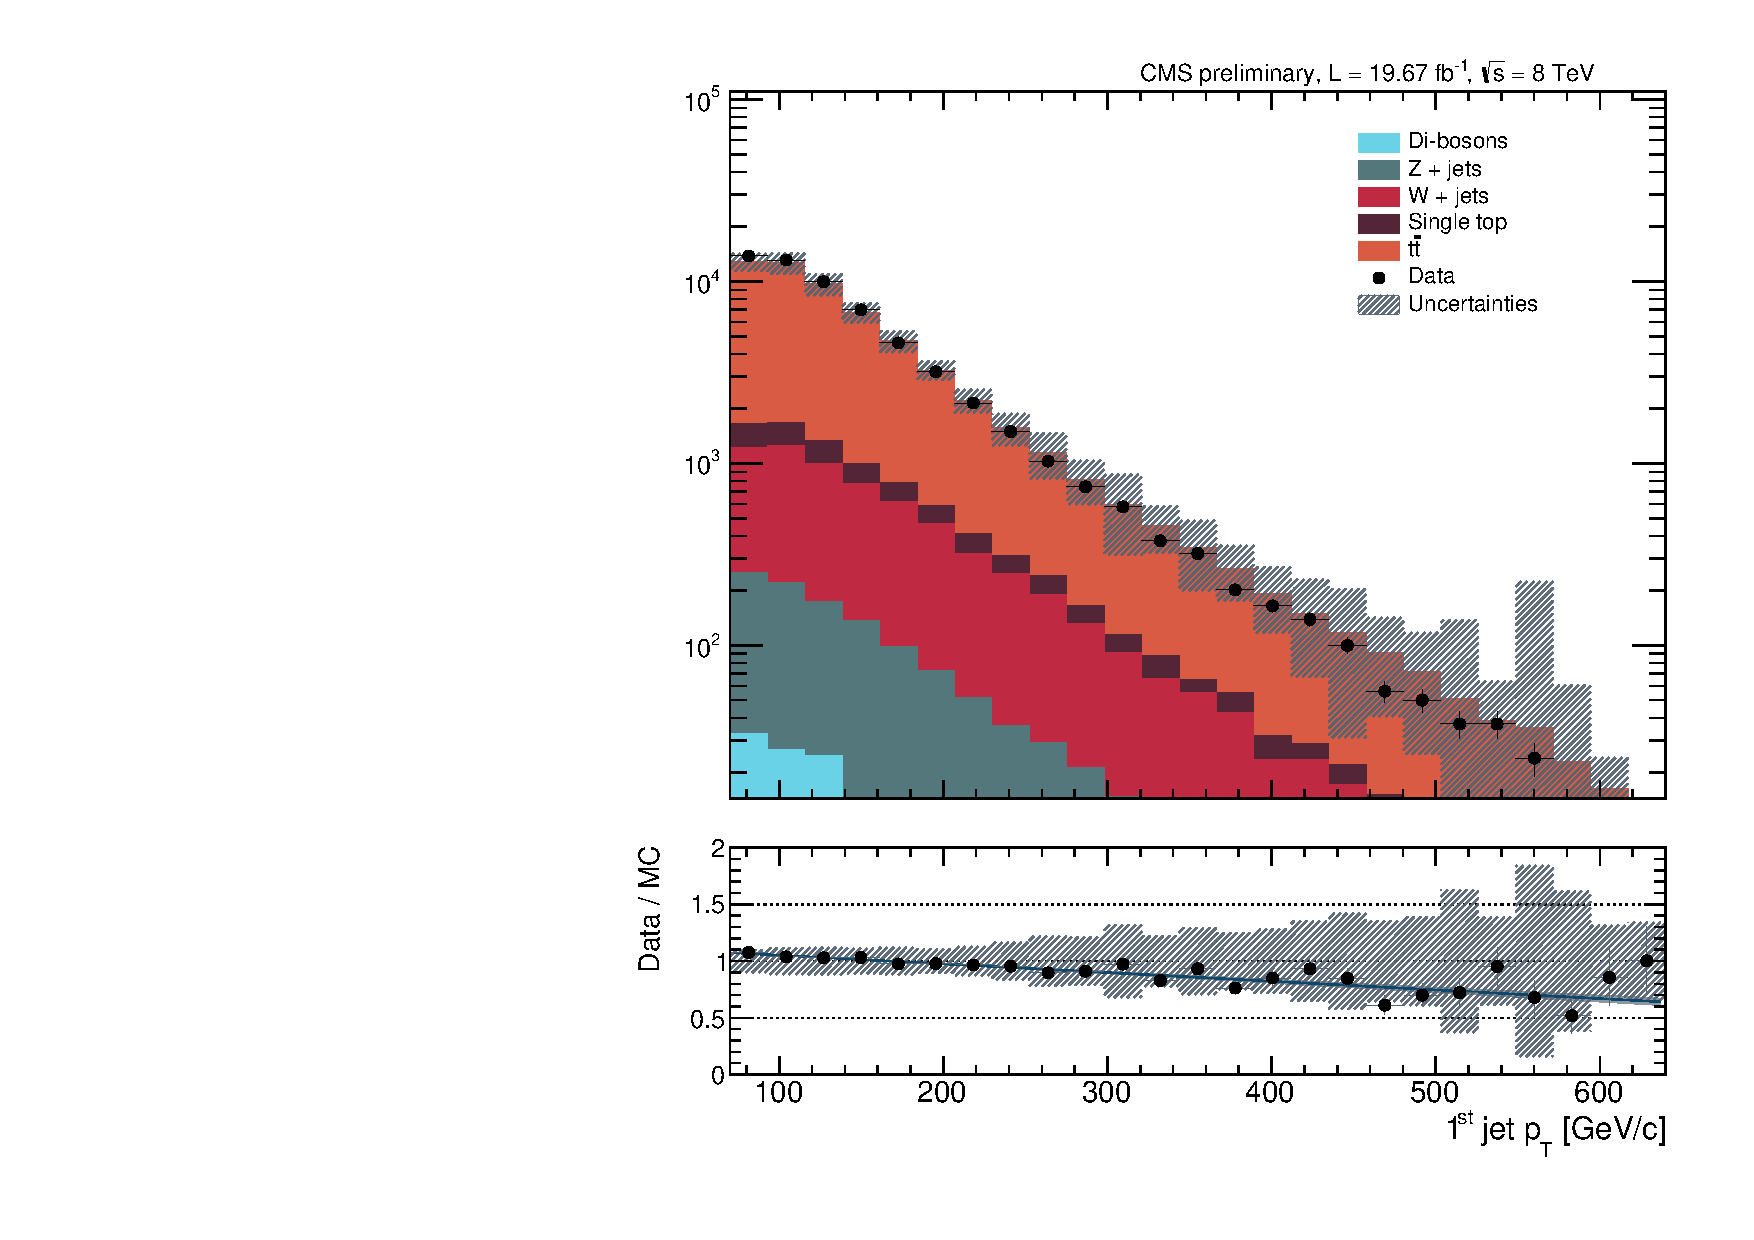
\includegraphics[width=0.49\textwidth,angle=-90,origin=c]{annexes/figs/higgs/data_mc/1-btag/semie/firstJetPt_reco_fullsel.pdf}}
    \captionsetup{format=plain,indention=0.2cm,font=small,labelfont={sf,bf},justification=justified}
    \caption{Comparaison entre les données et la simulation de l'impulsion transverse du premier jet sélectionné. Un ratio est présenté en bas de la distribution. La simulation est normalisée au nombre d'événements dans les données, en utilisant des facteurs de correction extraits d'un ajustement par la méthode du maximum de vraisemblance. La zone hachurée correspond aux incertitudes statistiques + systématiques.}
    \label{fig:higgs_data_mc_1jet}
\end{figure}

% \begin{figure}[p!] \centering
%     \captionsetup{format=plain,indention=0.2cm,font=small,labelfont={sf,bf},justification=centering}
%     \subcaptionbox{Canal semi-muonique,\\au moins 2 jets étiquetés \Pbottom}[0.49\textwidth]{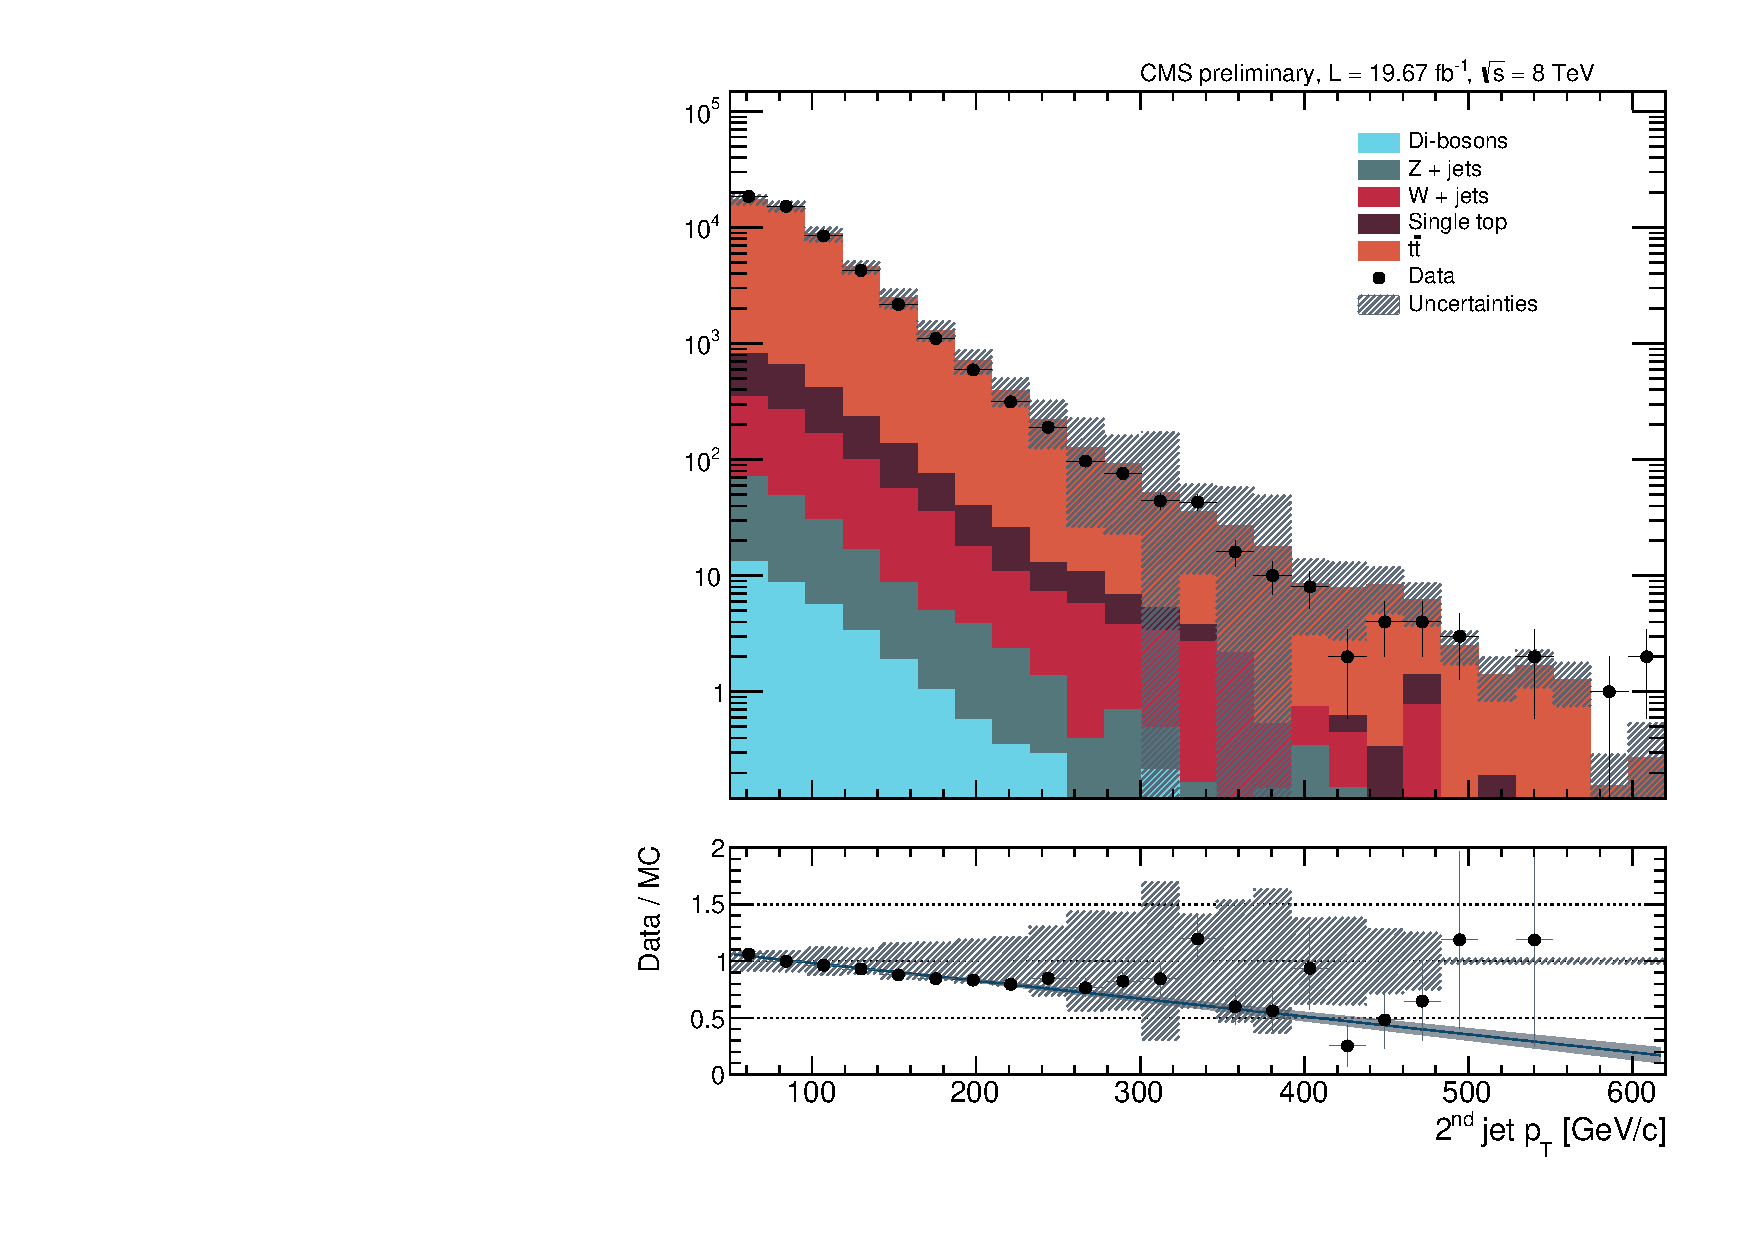
\includegraphics[width=0.49\textwidth,angle=-90,origin=c]{annexes/figs/higgs/data_mc/2-btag/semimu/secondJetPt_reco_fullsel.pdf}} \hfill
%     \subcaptionbox{Canal semi-électronique,\\au moins 2 jets étiquetés \Pbottom}[0.49\textwidth]{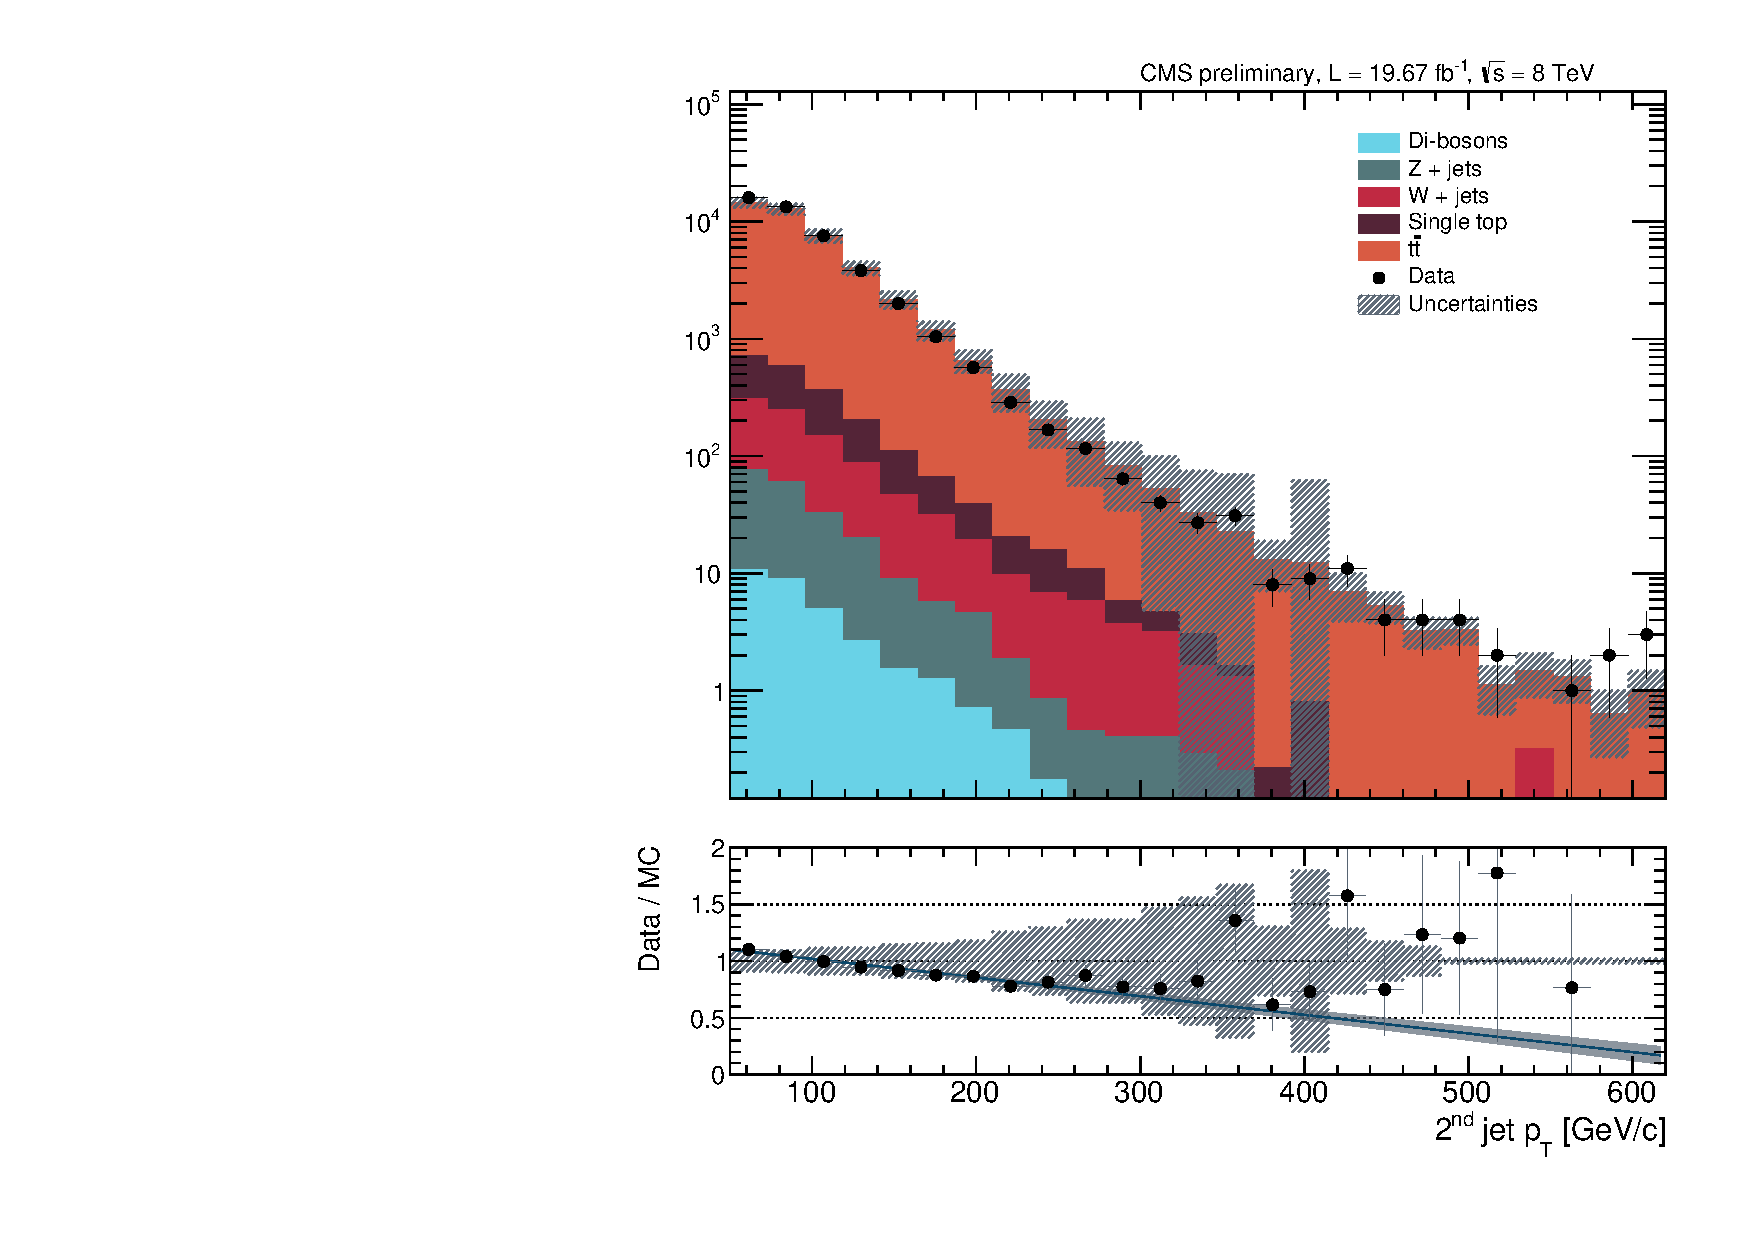
\includegraphics[width=0.49\textwidth,angle=-90,origin=c]{annexes/figs/higgs/data_mc/2-btag/semie/secondJetPt_reco_fullsel.pdf}} \\ \vspace{5mm}
%     \subcaptionbox{Canal semi-muonique,\\exactement 1 jet étiqueté \Pbottom}[0.49\textwidth]{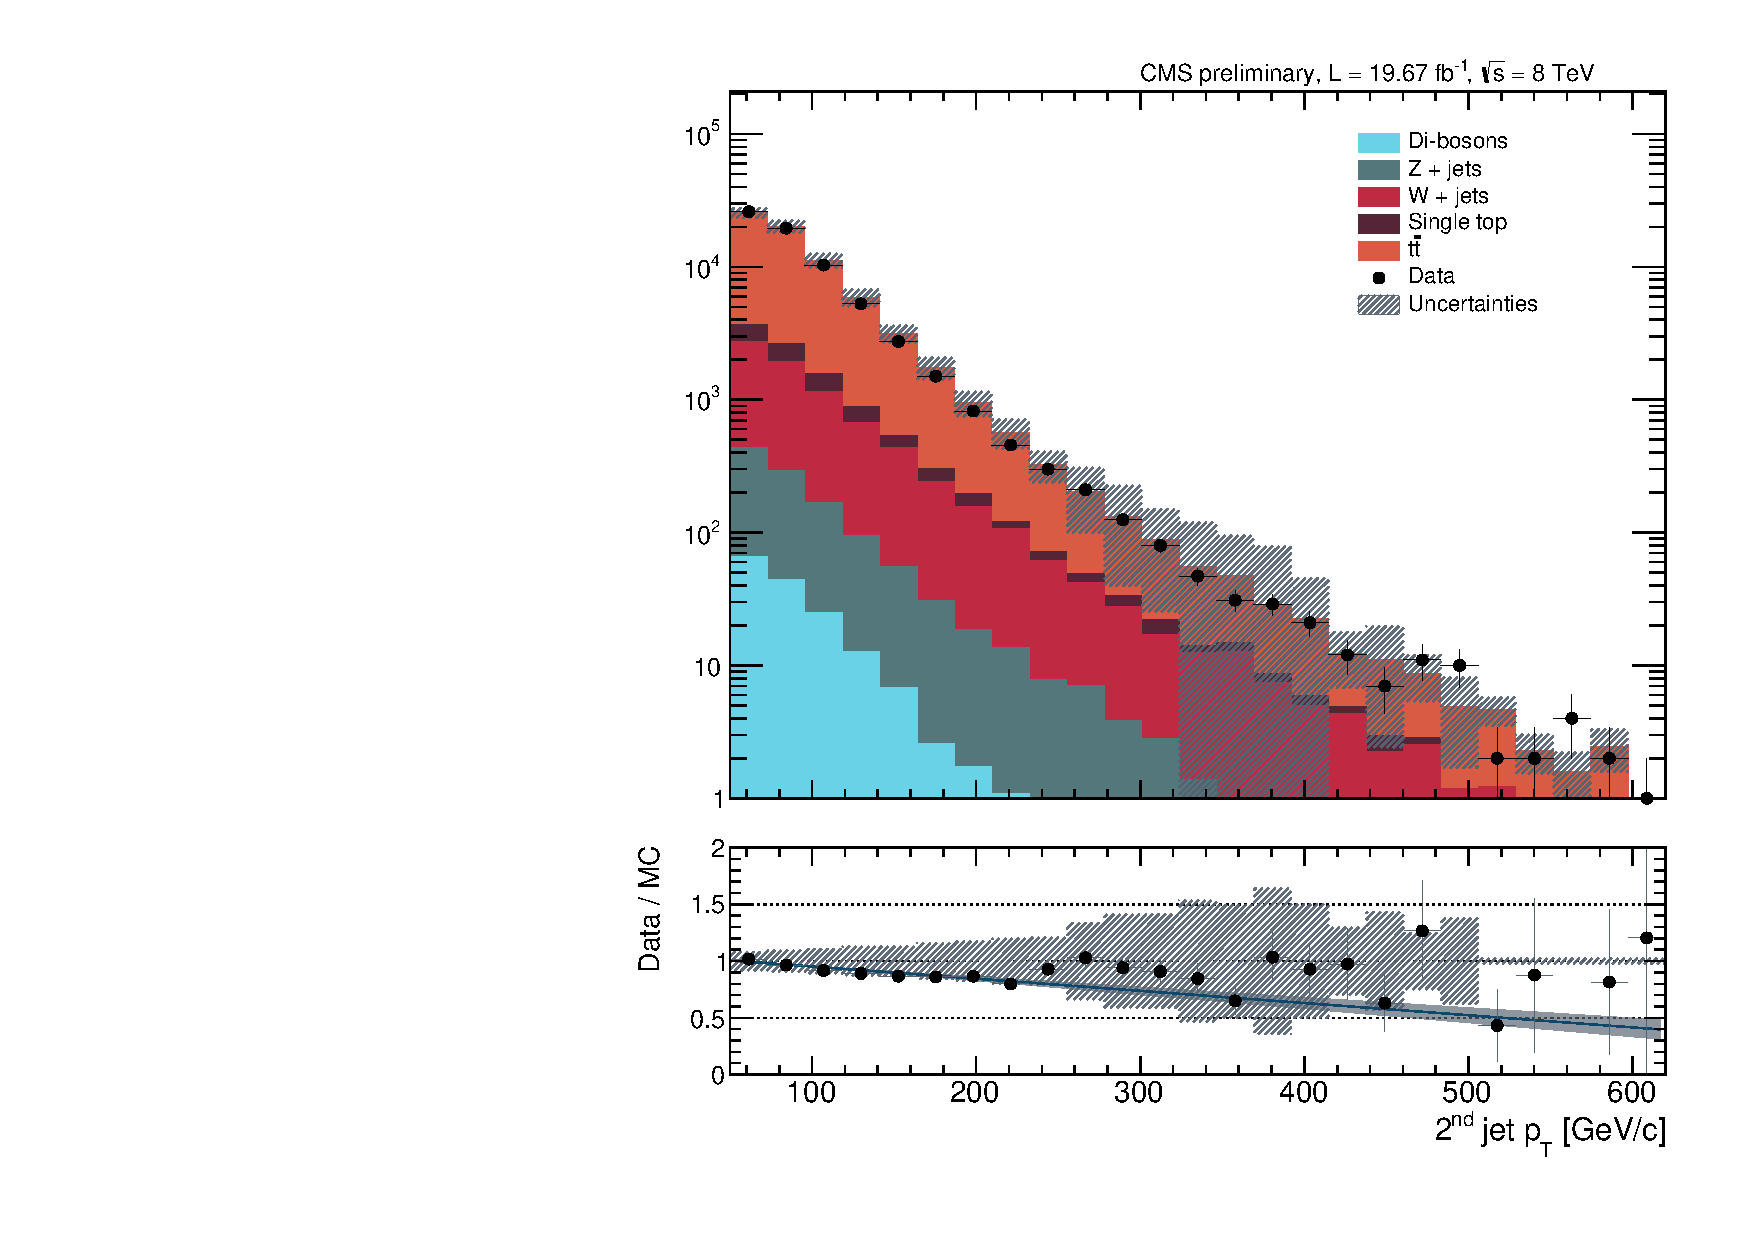
\includegraphics[width=0.49\textwidth,angle=-90,origin=c]{annexes/figs/higgs/data_mc/1-btag/semimu/secondJetPt_reco_fullsel.pdf}} \hfill
%     \subcaptionbox{Canal semi-électronique,\\exactement 1 jet étiqueté \Pbottom}[0.49\textwidth]{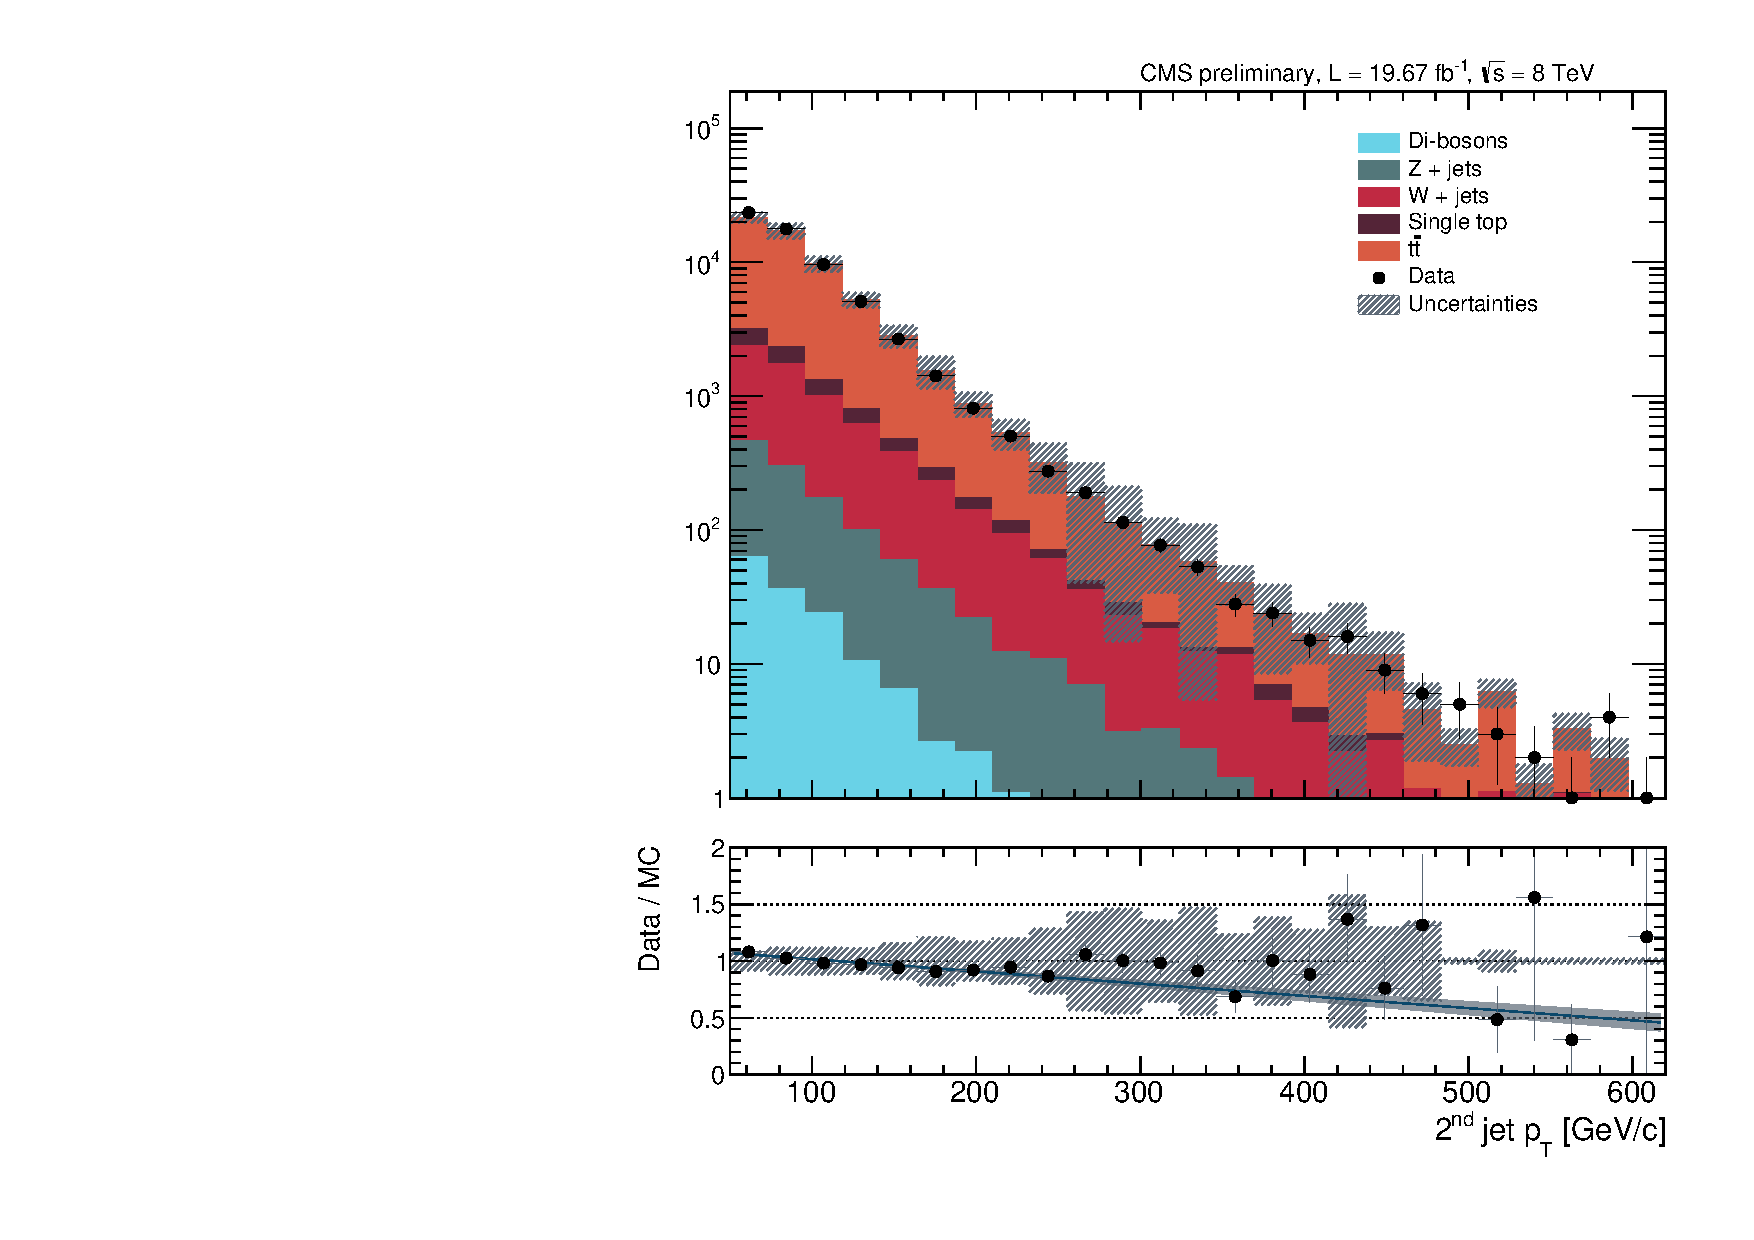
\includegraphics[width=0.49\textwidth,angle=-90,origin=c]{annexes/figs/higgs/data_mc/1-btag/semie/secondJetPt_reco_fullsel.pdf}}
%     \captionsetup{format=plain,indention=0.2cm,font=small,labelfont={sf,bf},justification=justified}
%     \caption{Comparaison entre les données et la simulation de l'impulsion transverse du second jet sélectionné. Un ratio est présenté en bas de la distribution. La simulation est normalisée au nombre d'événements dans les données, en utilisant des facteurs de correction extraits d'un ajustement par la méthode du maximum de vraisemblance. La zone hachurée correspond aux incertitudes statistiques + systématiques.}
%     \label{fig:higgs_data_mc_2jet}
% \end{figure}

\begin{figure}[p!] \centering
    \captionsetup{format=plain,indention=0.2cm,font=small,labelfont={sf,bf},justification=centering}
    \subcaptionbox{Canal semi-muonique,\\au moins 2 jets étiquetés \Pbottom}[0.49\textwidth]{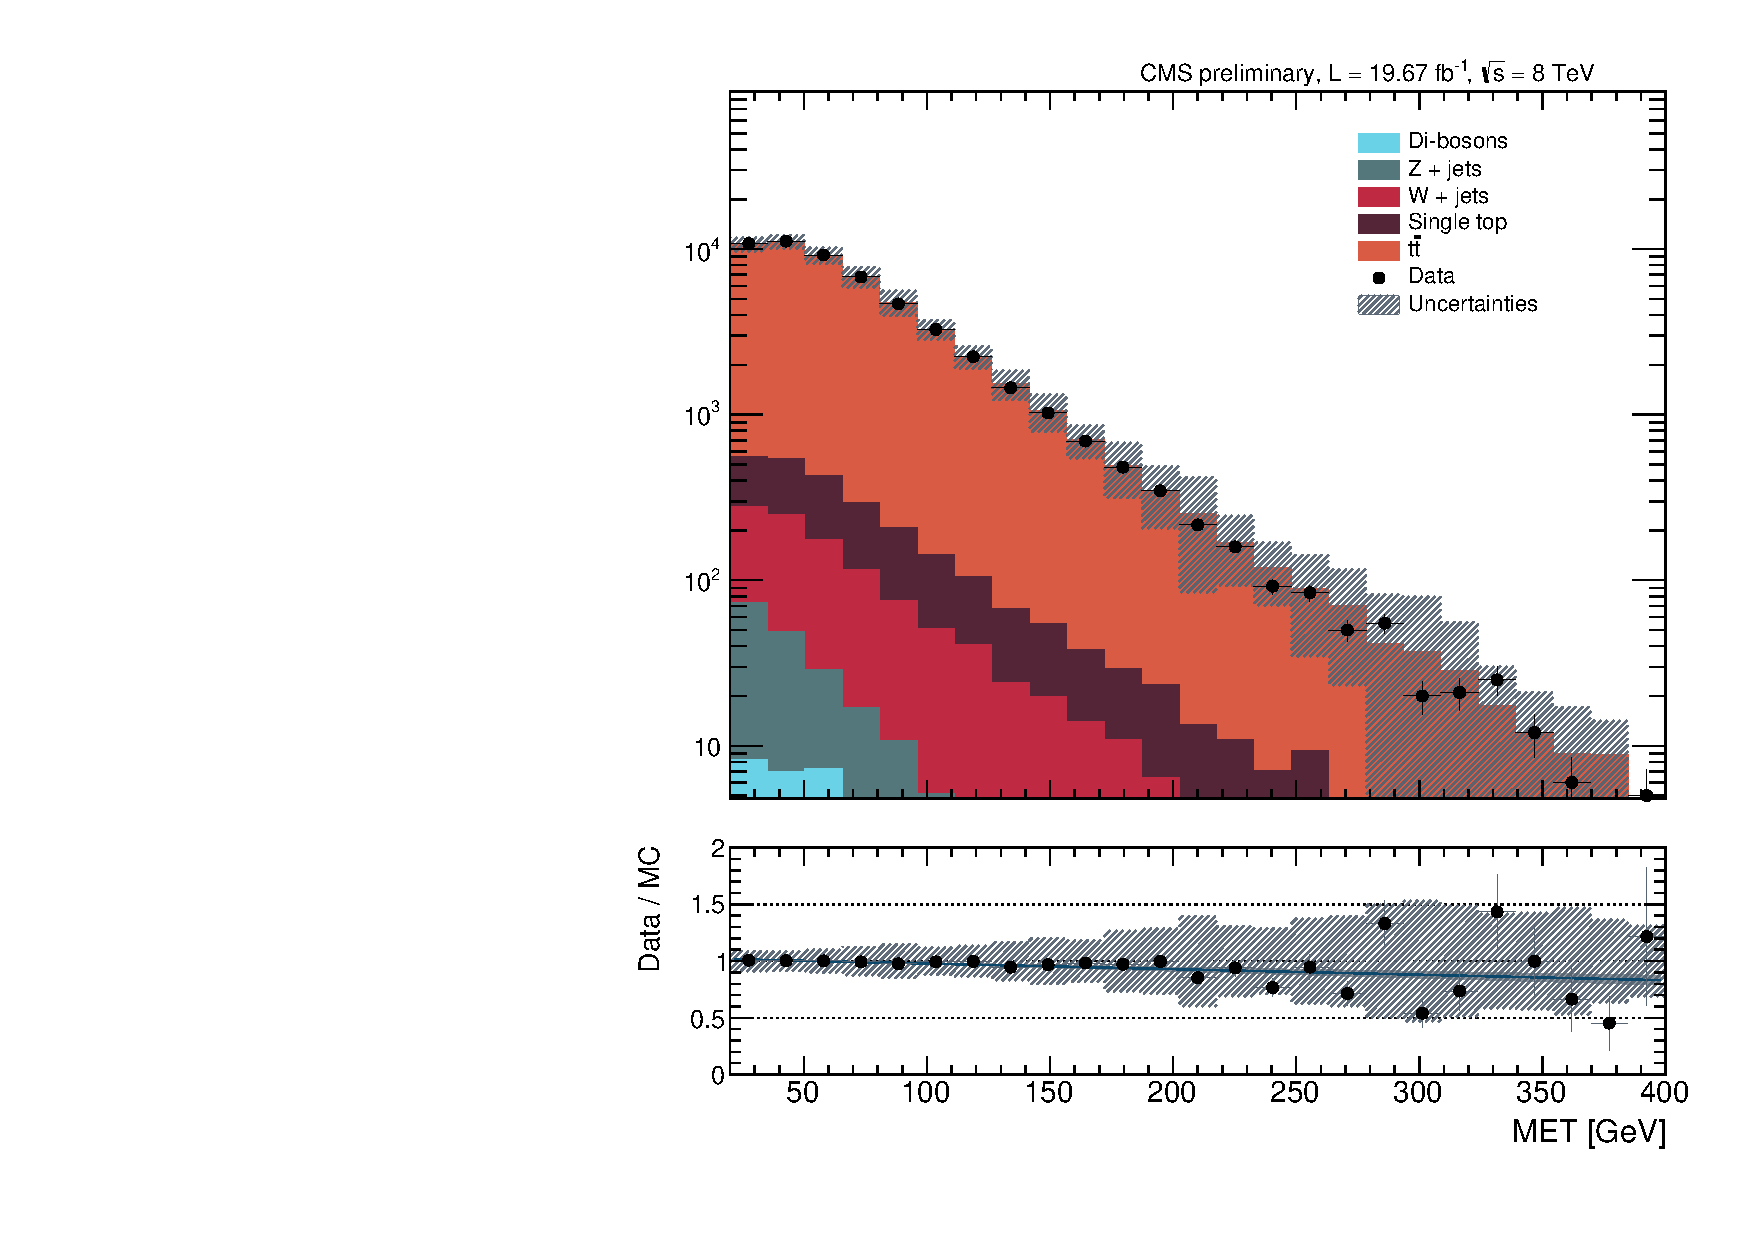
\includegraphics[width=0.49\textwidth,angle=-90,origin=c]{annexes/figs/higgs/data_mc/2-btag/semimu/MET_reco_fullsel.pdf}} \hfill
    \subcaptionbox{Canal semi-électronique,\\au moins 2 jets étiquetés \Pbottom}[0.49\textwidth]{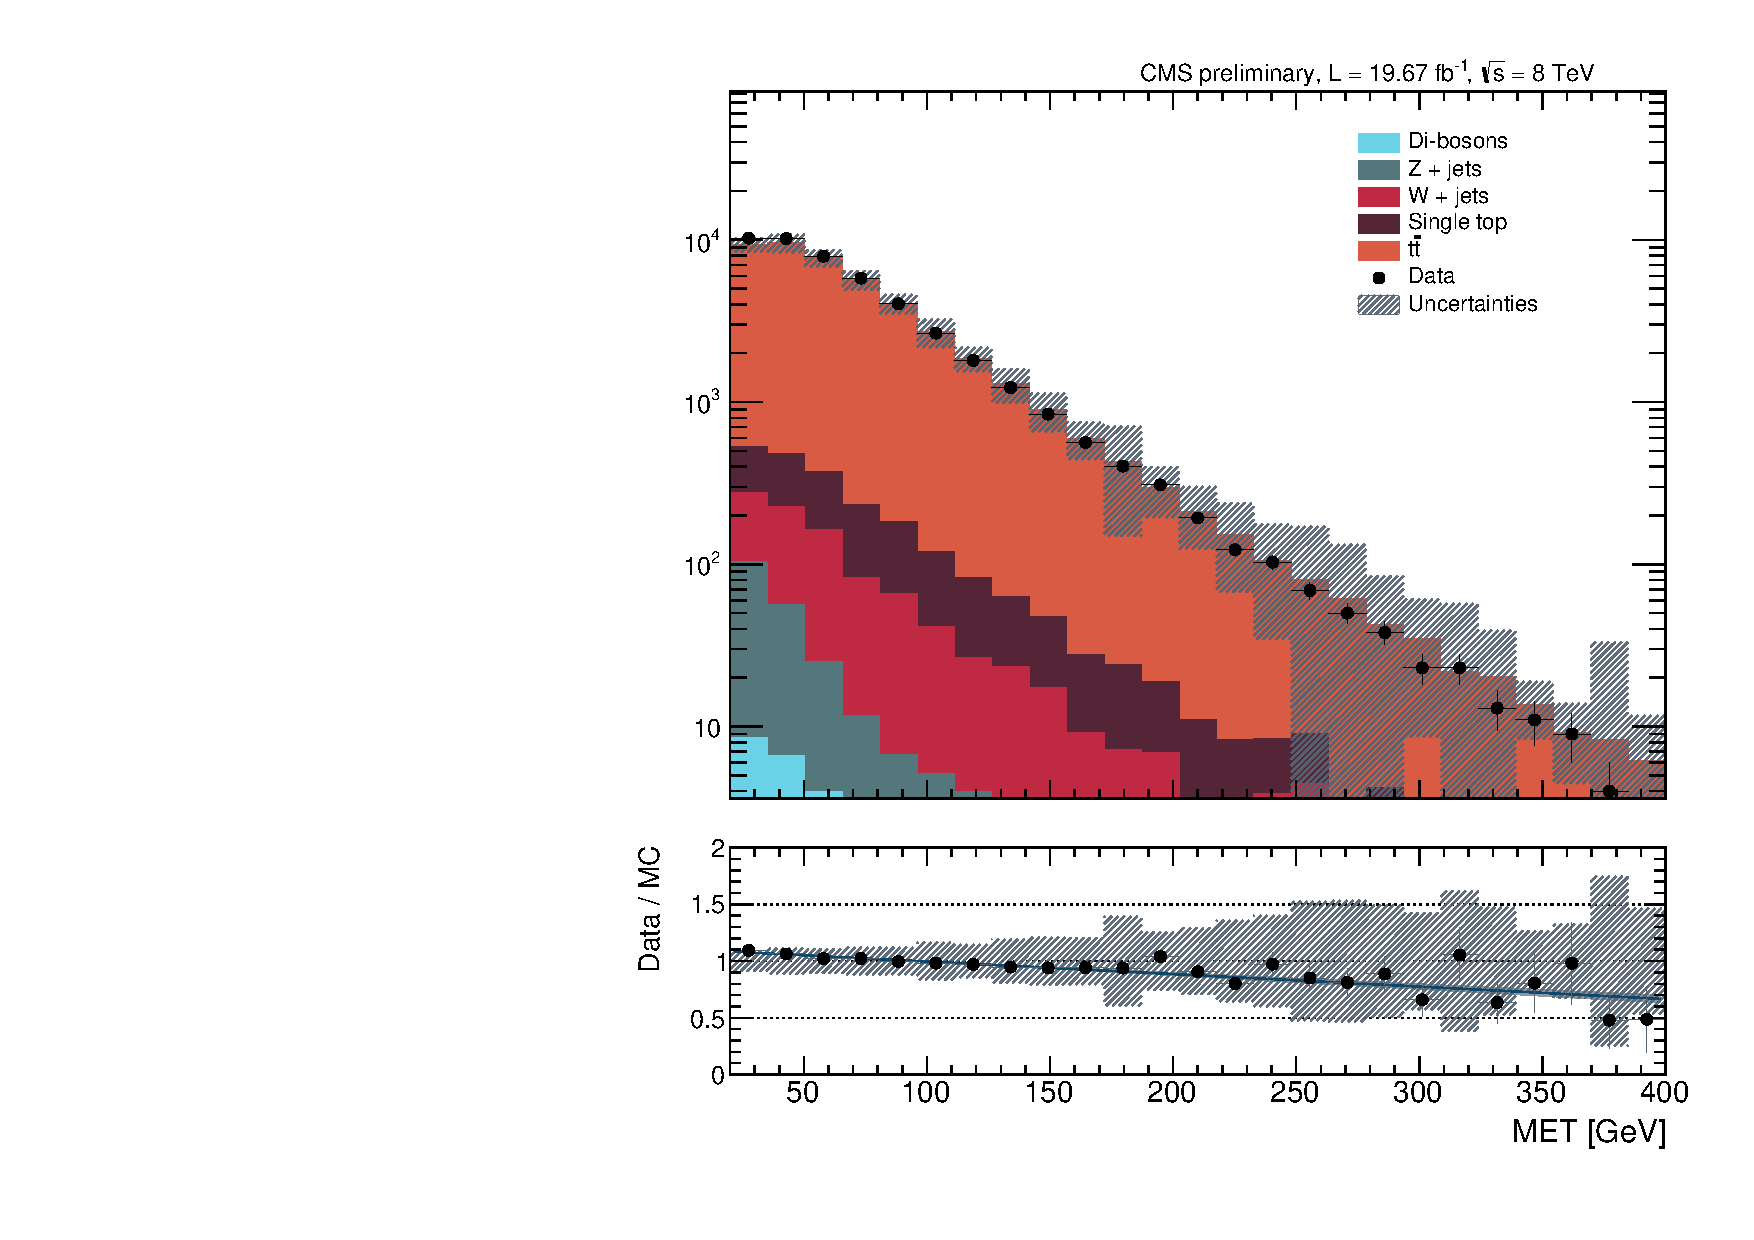
\includegraphics[width=0.49\textwidth,angle=-90,origin=c]{annexes/figs/higgs/data_mc/2-btag/semie/MET_reco_fullsel.pdf}} \\ \vspace{5mm}
    \subcaptionbox{Canal semi-muonique,\\exactement 1 jet étiqueté \Pbottom}[0.49\textwidth]{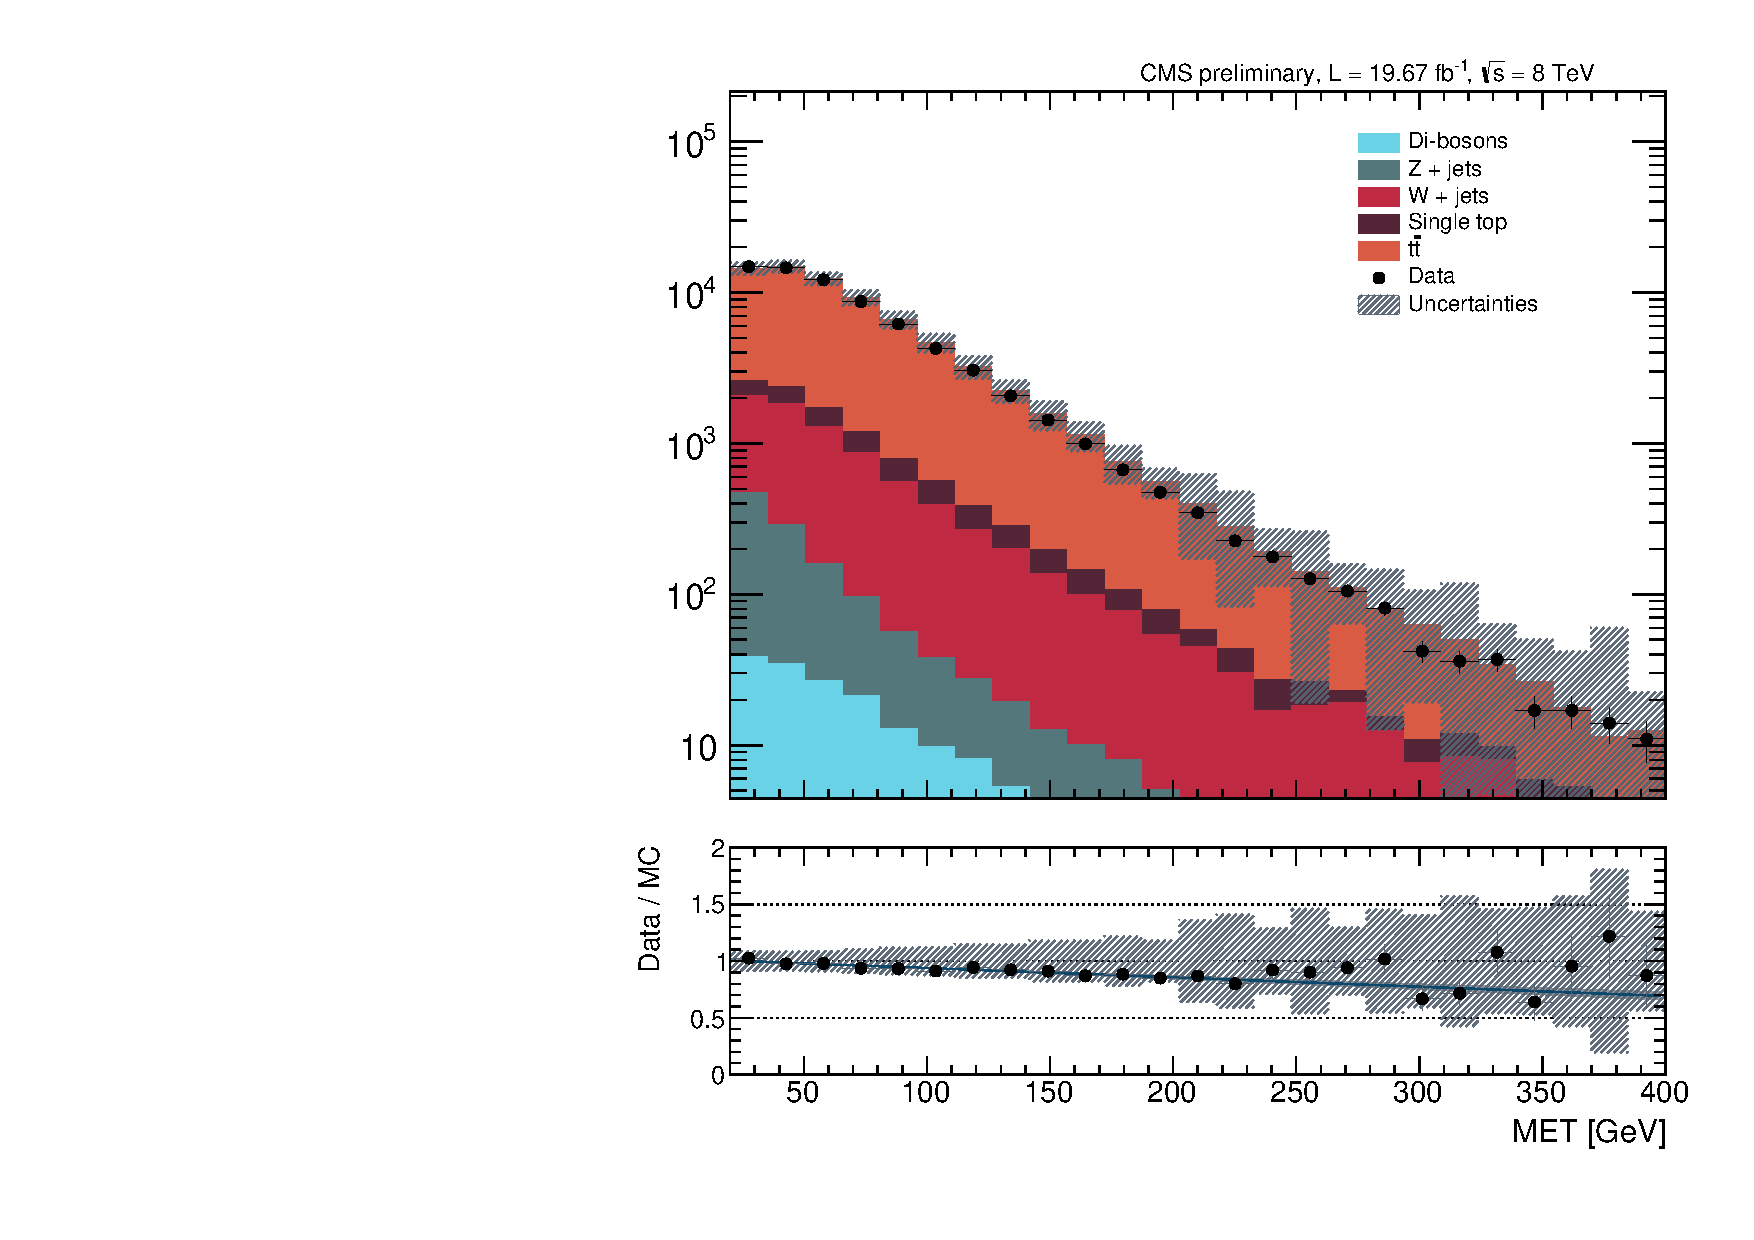
\includegraphics[width=0.49\textwidth,angle=-90,origin=c]{annexes/figs/higgs/data_mc/1-btag/semimu/MET_reco_fullsel.pdf}} \hfill
    \subcaptionbox{Canal semi-électronique,\\exactement 1 jet étiqueté \Pbottom}[0.49\textwidth]{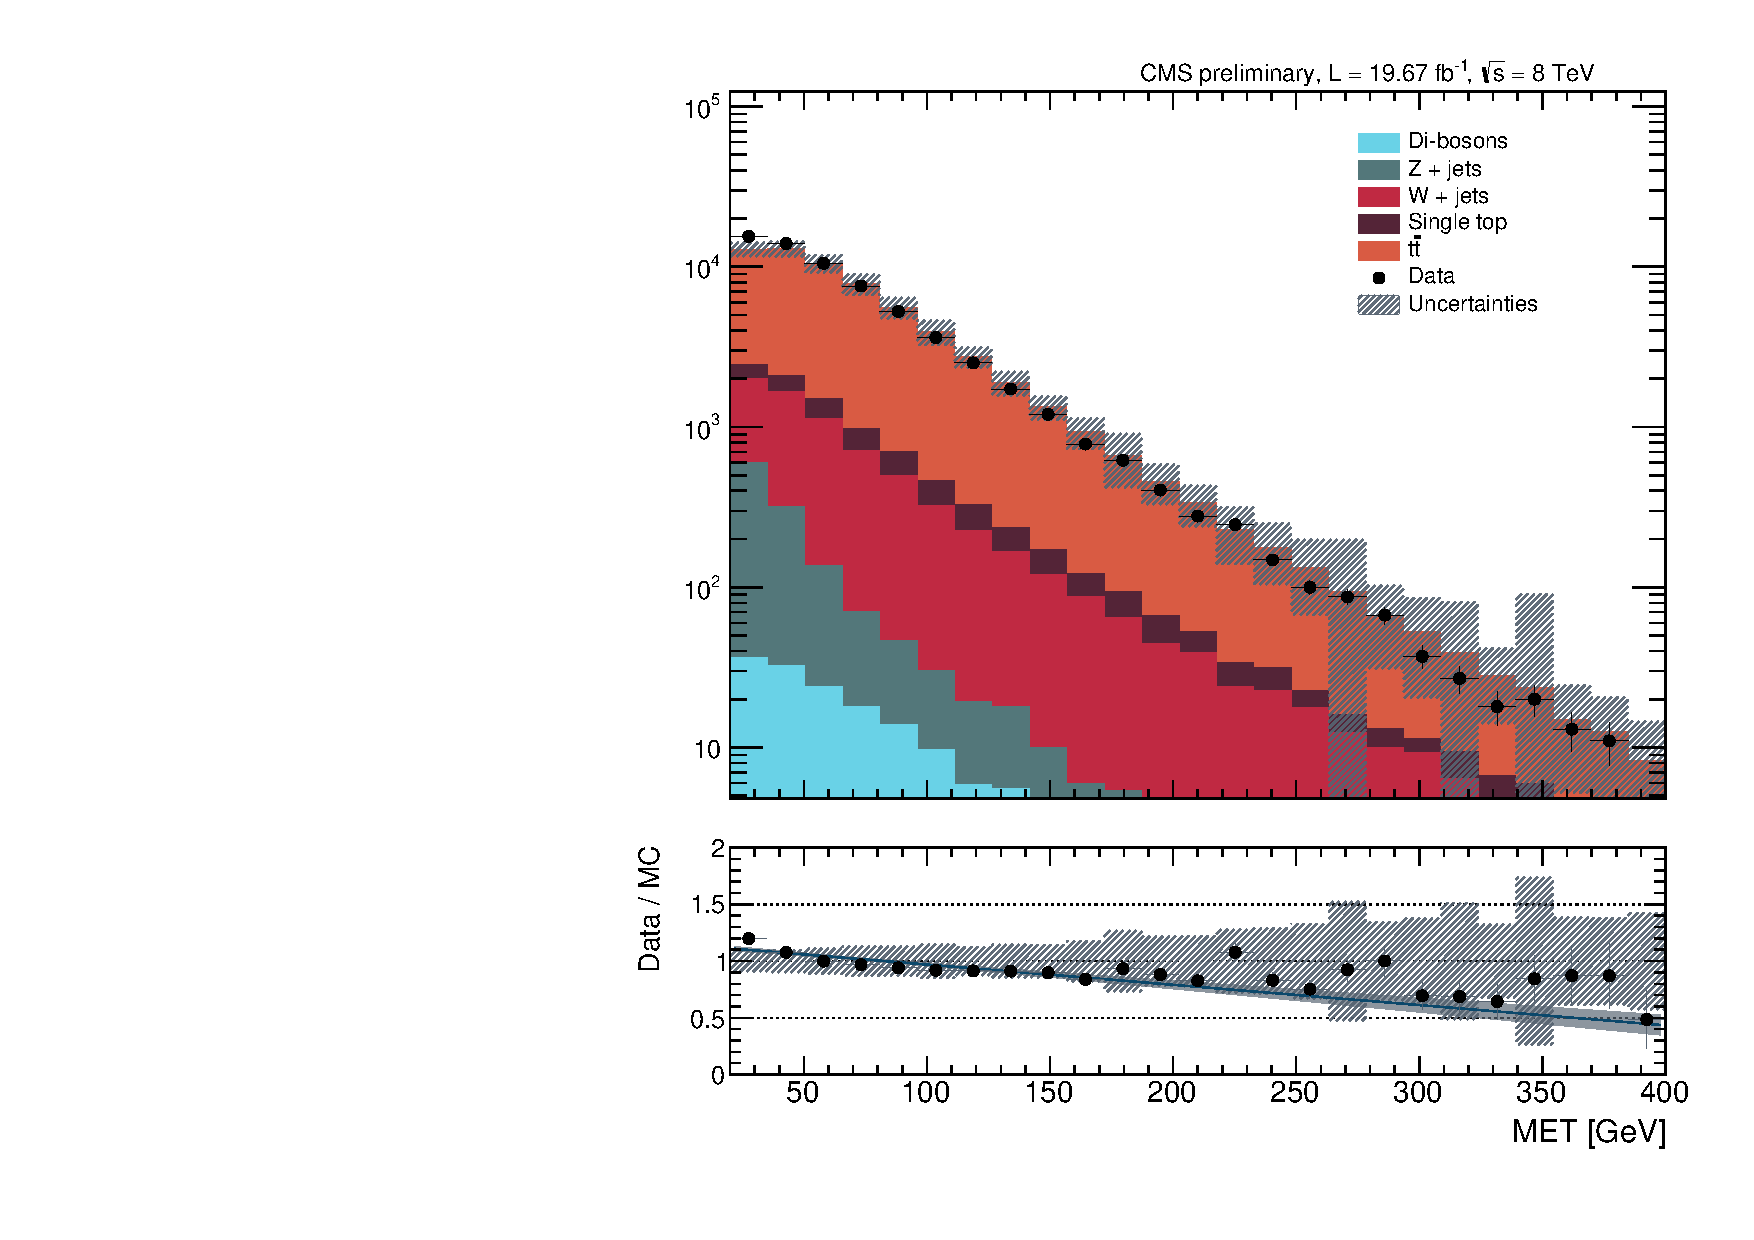
\includegraphics[width=0.49\textwidth,angle=-90,origin=c]{annexes/figs/higgs/data_mc/1-btag/semie/MET_reco_fullsel.pdf}}
    \captionsetup{format=plain,indention=0.2cm,font=small,labelfont={sf,bf},justification=justified}
    \caption{Comparaison entre les données et la simulation de l'énergie transverse manquante. Un ratio est présenté en bas de la distribution. La simulation est normalisée au nombre d'événements dans les données, en utilisant des facteurs de correction extraits d'un ajustement par la méthode du maximum de vraisemblance. La zone hachurée correspond aux incertitudes statistiques + systématiques.}
    \label{fig:higgs_data_mc_met}
\end{figure}

\begin{figure}[p!] \centering
    \captionsetup{format=plain,indention=0.2cm,font=small,labelfont={sf,bf},justification=centering}
    \subcaptionbox{Canal semi-muonique,\\au moins 2 jets étiquetés \Pbottom}[0.49\textwidth]{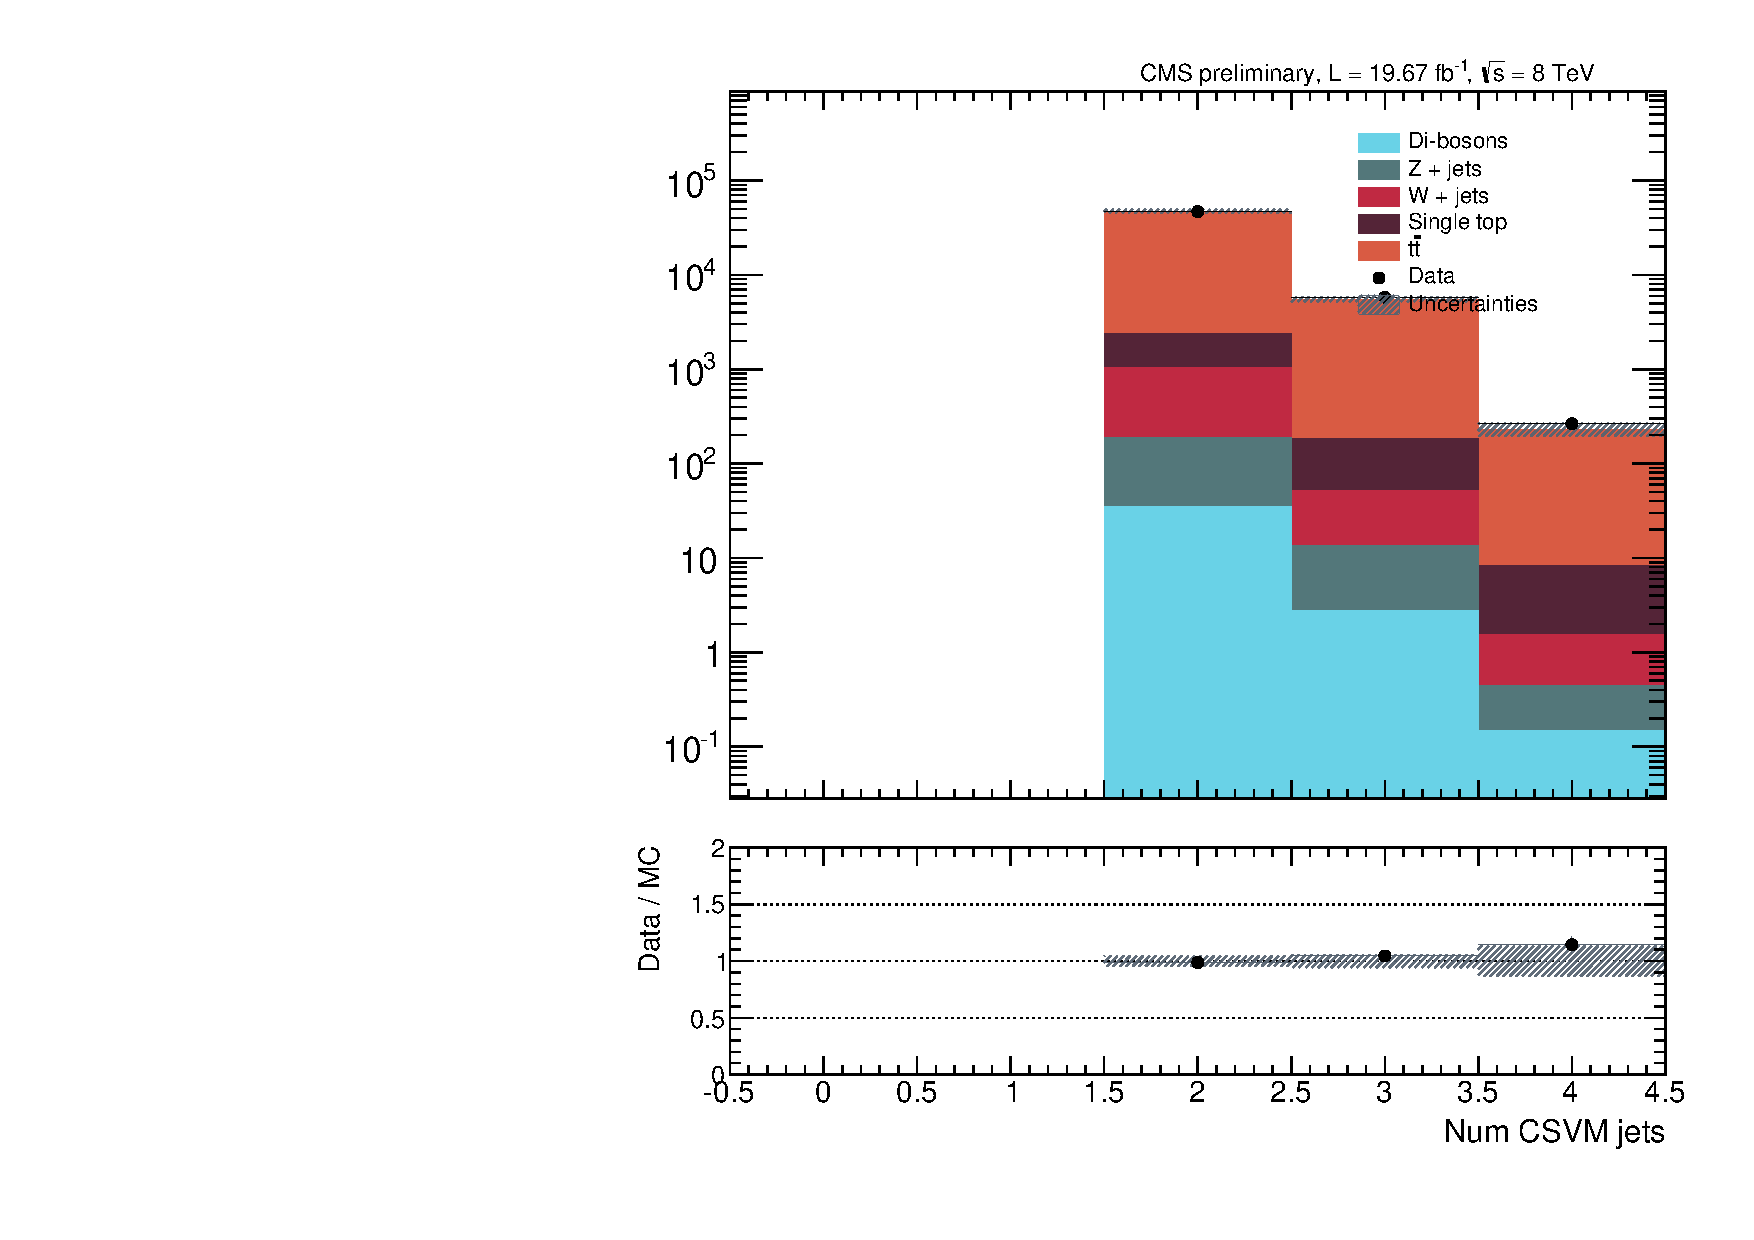
\includegraphics[width=0.49\textwidth,angle=-90,origin=c]{annexes/figs/higgs/data_mc/2-btag/semimu/nBTaggedJets_reco_fullsel.pdf}} \hfill
    \subcaptionbox{Canal semi-électronique,\\au moins 2 jets étiquetés \Pbottom}[0.49\textwidth]{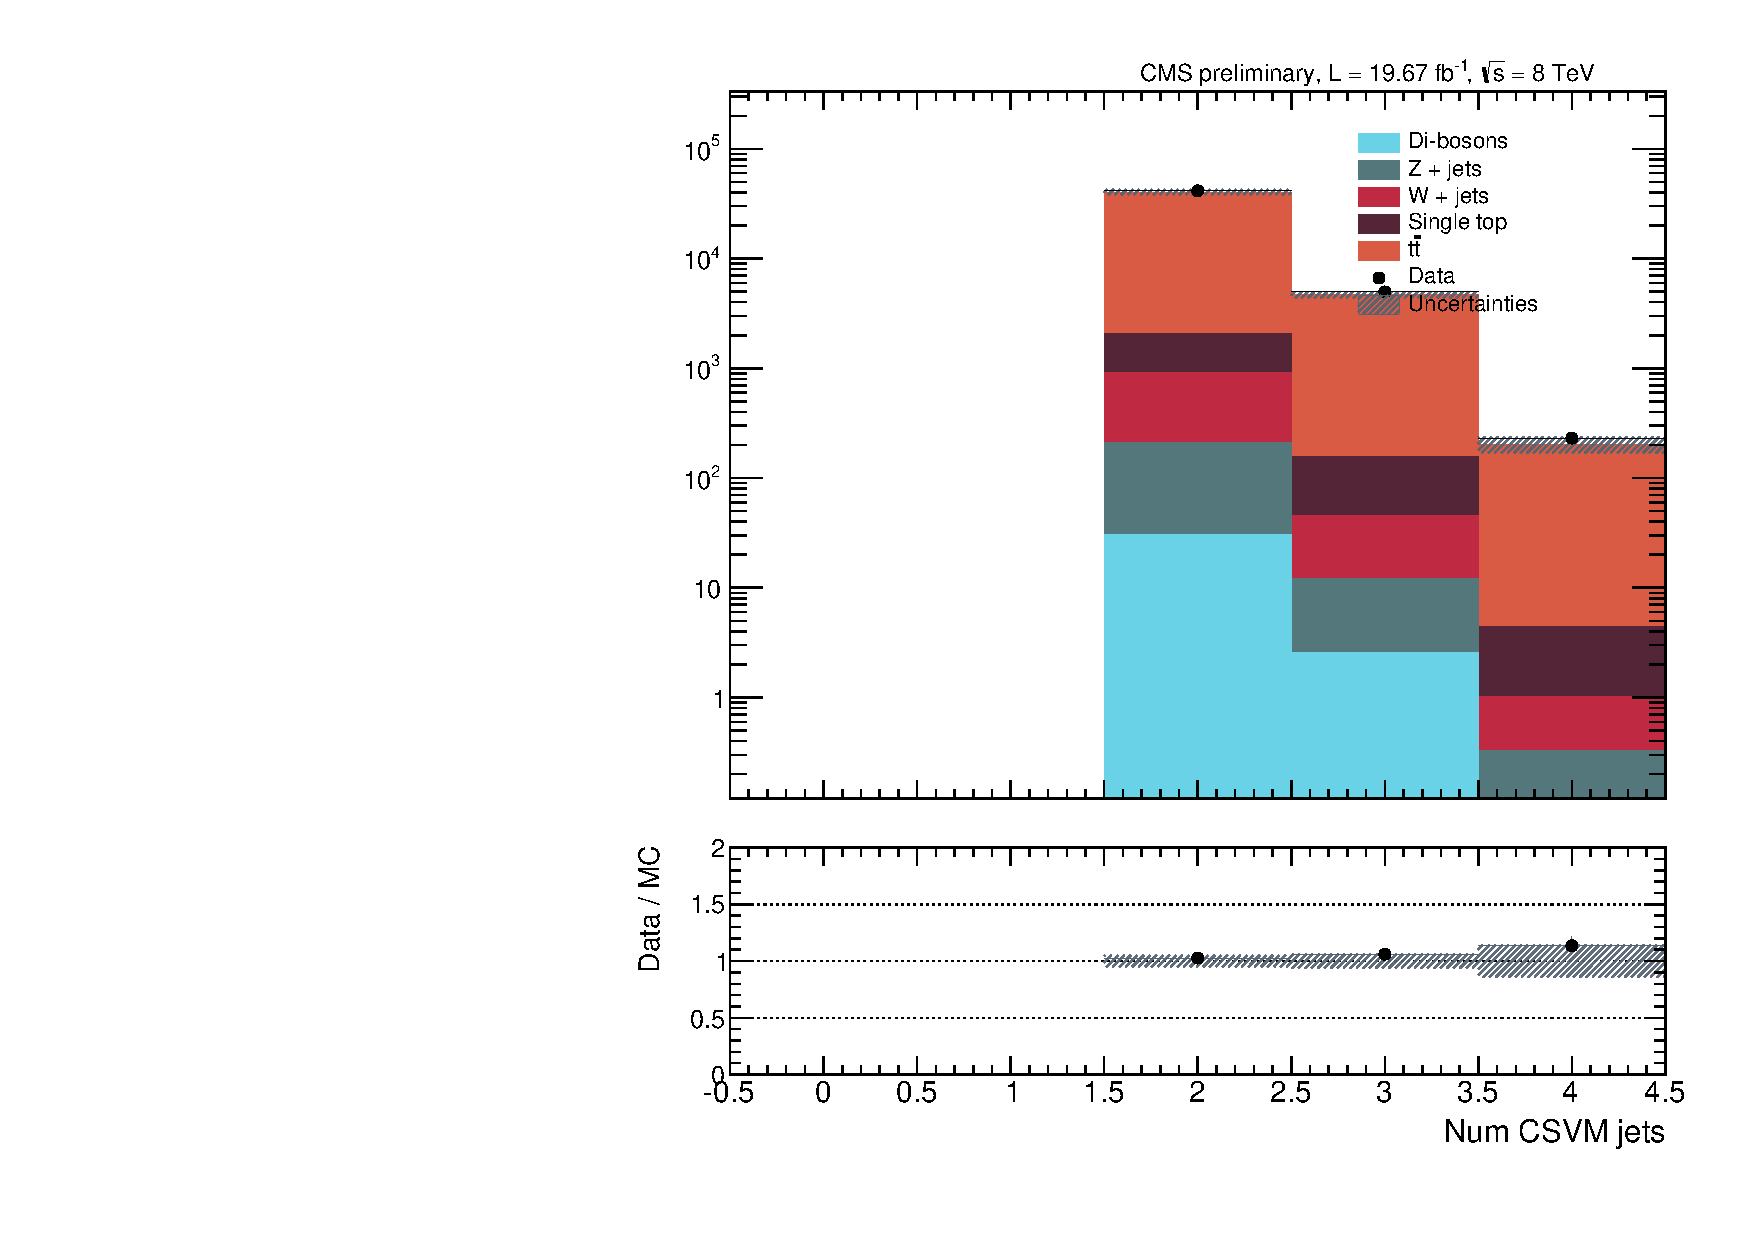
\includegraphics[width=0.49\textwidth,angle=-90,origin=c]{annexes/figs/higgs/data_mc/2-btag/semie/nBTaggedJets_reco_fullsel.pdf}} \\ \vspace{5mm}
    \subcaptionbox{Canal semi-muonique,\\exactement 1 jet étiqueté \Pbottom}[0.49\textwidth]{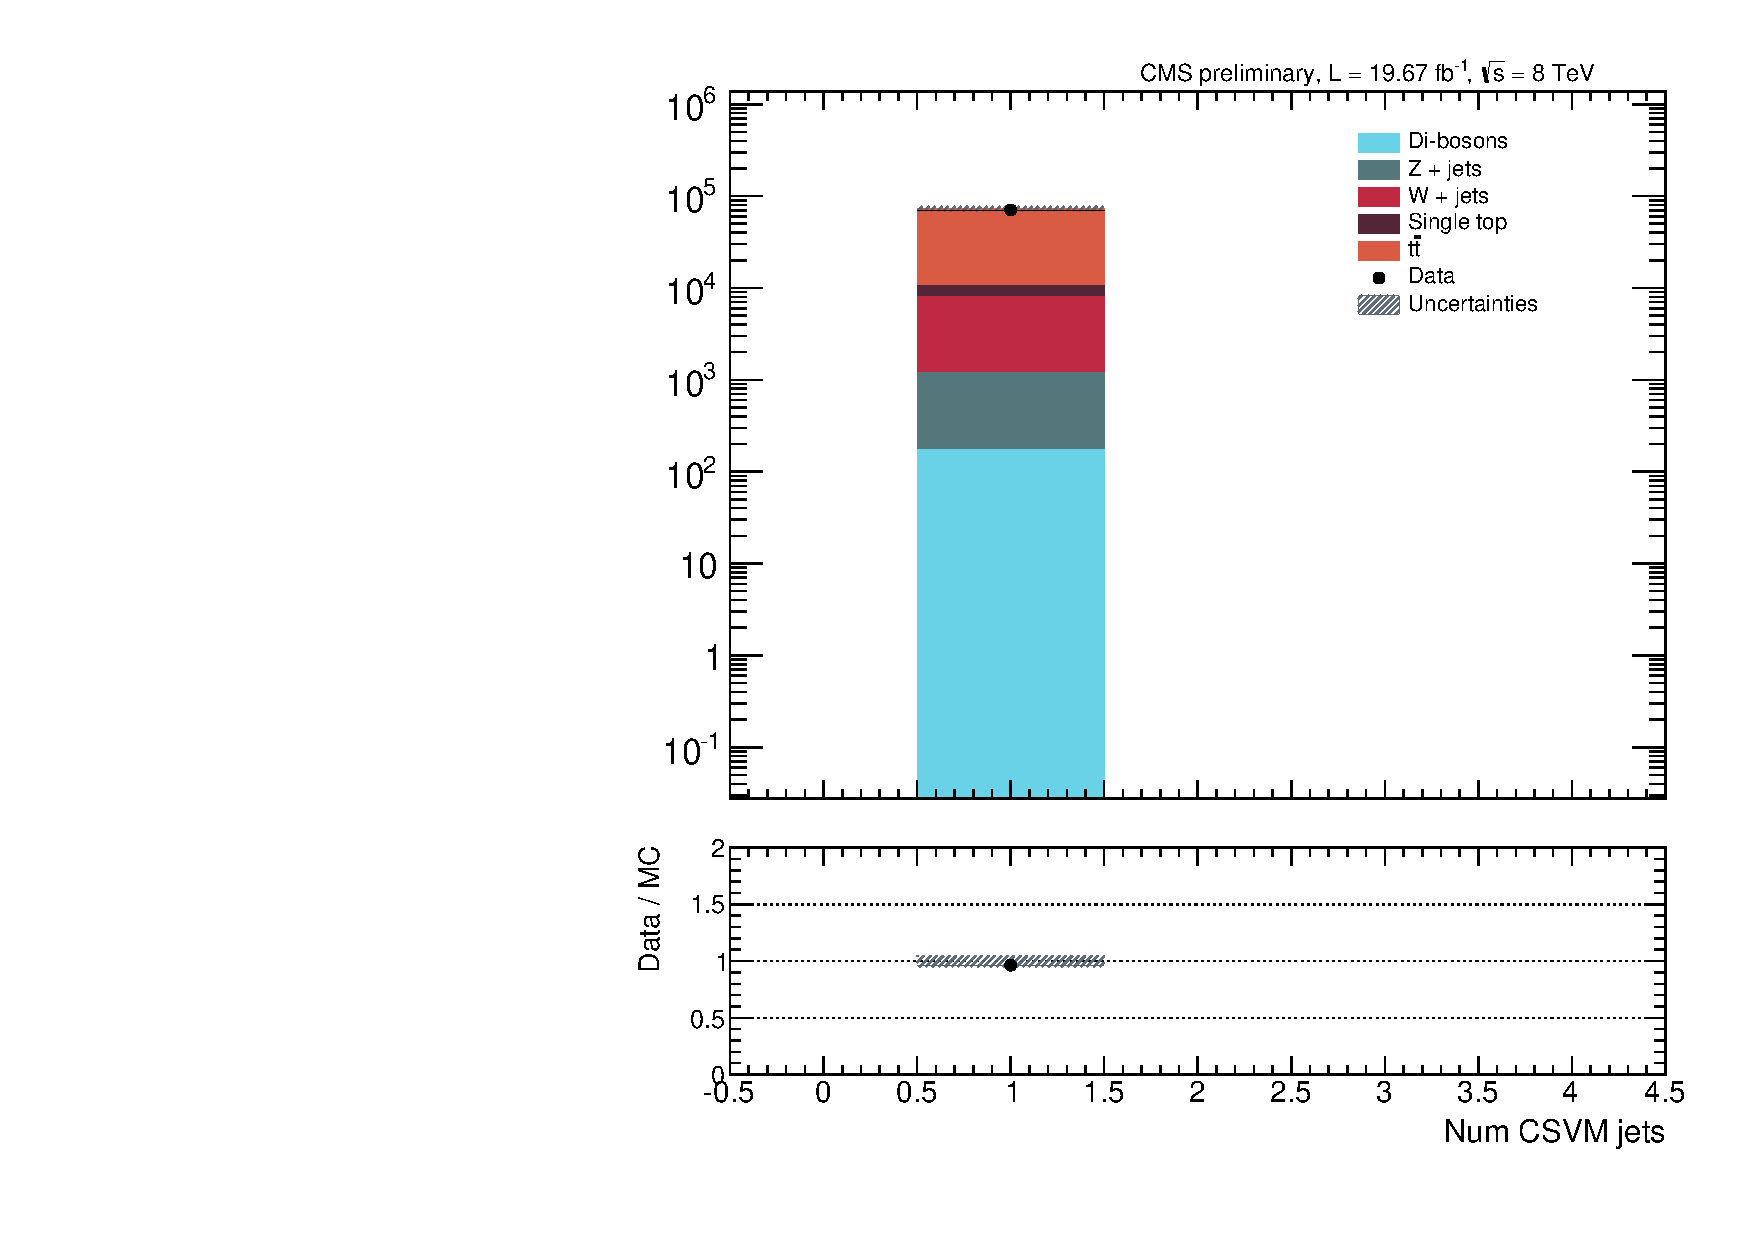
\includegraphics[width=0.49\textwidth,angle=-90,origin=c]{annexes/figs/higgs/data_mc/1-btag/semimu/nBTaggedJets_reco_fullsel.pdf}} \hfill
    \subcaptionbox{Canal semi-électronique,\\exactement 1 jet étiqueté \Pbottom}[0.49\textwidth]{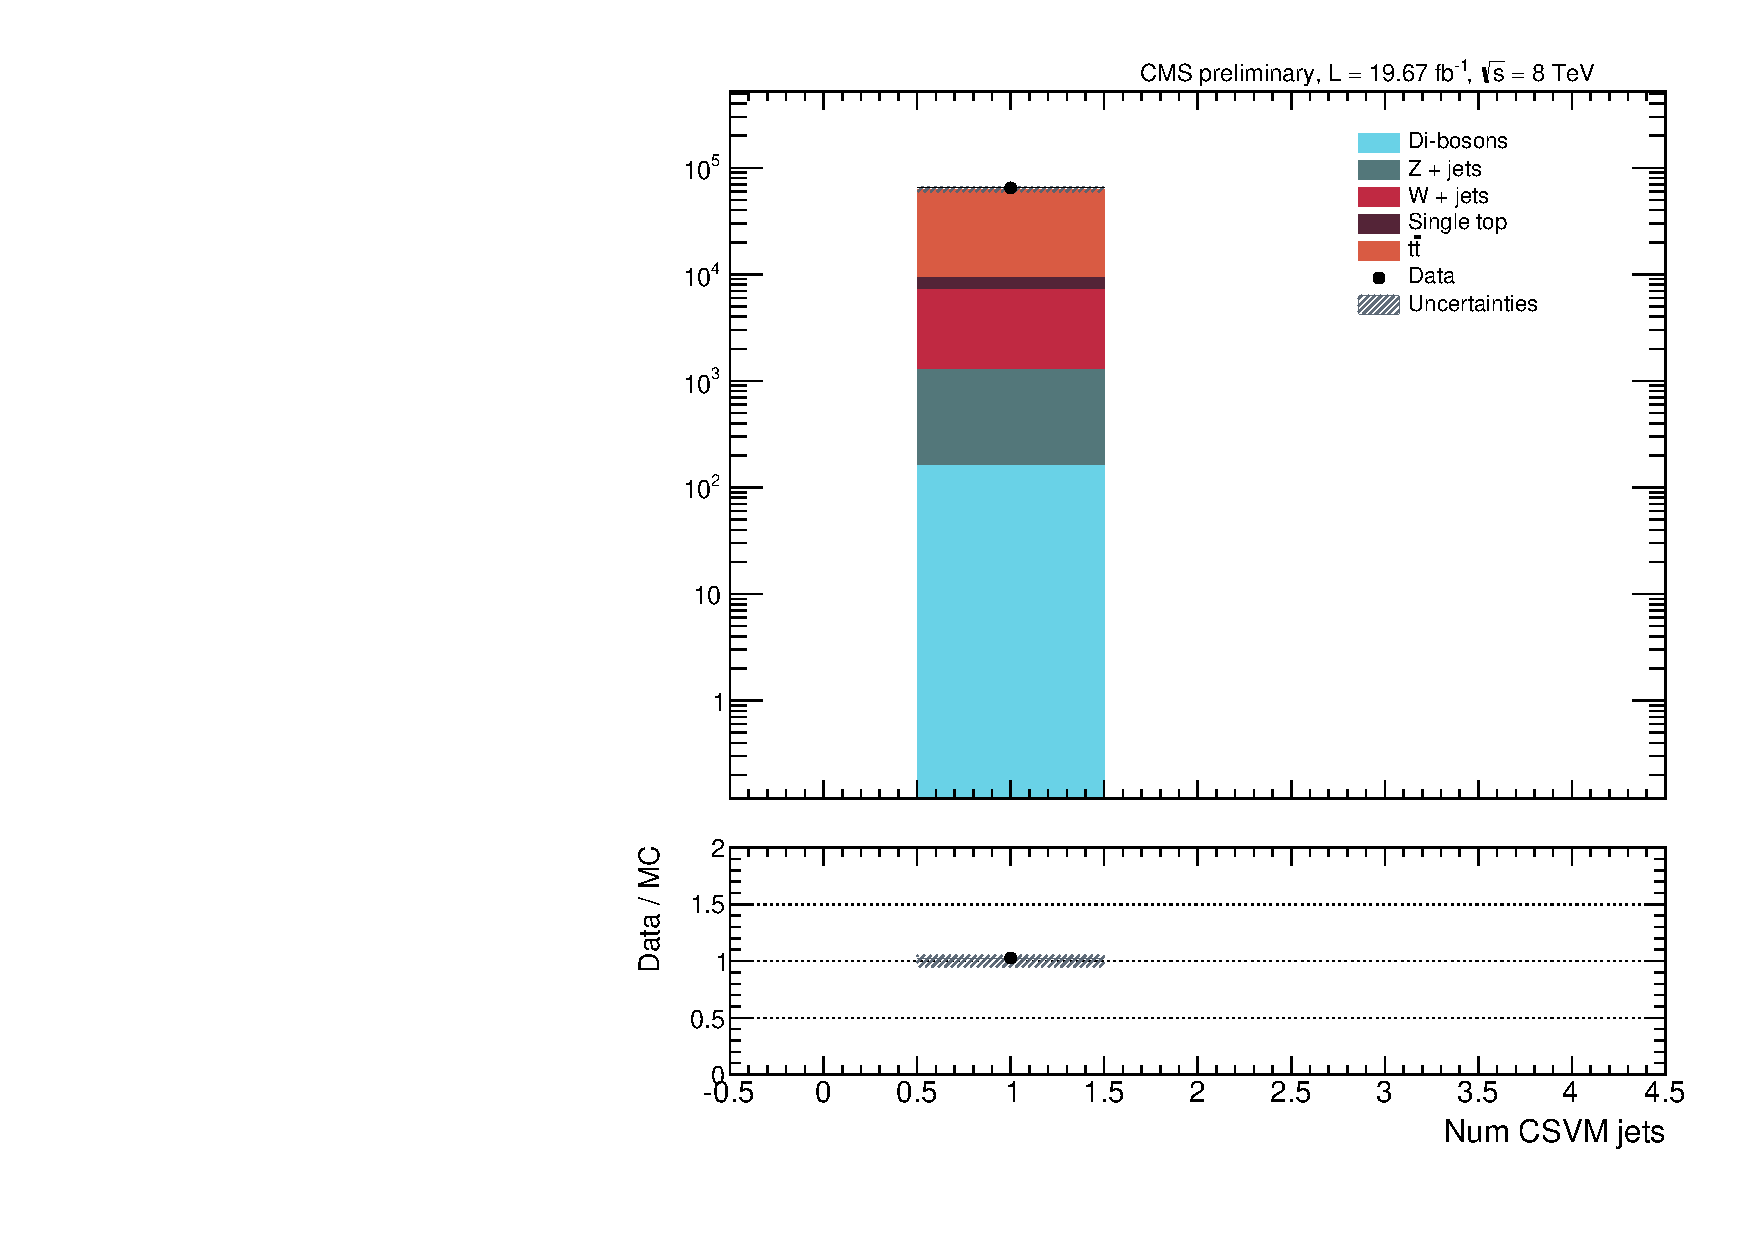
\includegraphics[width=0.49\textwidth,angle=-90,origin=c]{annexes/figs/higgs/data_mc/1-btag/semie/nBTaggedJets_reco_fullsel.pdf}}
    \captionsetup{format=plain,indention=0.2cm,font=small,labelfont={sf,bf},justification=justified}
    \caption{Comparaison entre les données et la simulation du nombre de jets étiquetés \Pbottom. Un ratio est présenté en bas de la distribution. La simulation est normalisée au nombre d'événements dans les données, en utilisant des facteurs de correction extraits d'un ajustement par la méthode du maximum de vraisemblance. La zone hachurée correspond aux incertitudes statistiques + systématiques.}
    \label{fig:higgs_data_mc_nb}
\end{figure}